% VLDB-Template enhances the ACM master template, acmart.cls v2.19 (2026/06/27):
% https://www.acm.org/publications/proceedings-template
% The ACM Latex guide provides further information about the ACM template
%
% This bundle pins acmart.cls v2.19 (rather than relying on whatever version
% ships with an author's local TeX install or Overleaf project) to guarantee
% consistent formatting across all PVLDB submissions.

\documentclass[sigconf, nonacm]{acmart}

%%% do not modify the following VLDB block %%
%%% VLDB block start %%%
\usepackage{pvldb}% VLDB/PVLDB formatting overrides, see pvldb.sty for details.
                      % Do not remove -- required for consistent proceedings
                      % formatting across all VLDB submissions.
%%% VLDB block end %%%

\usepackage{subcaption}

%% The following must be set for each paper (values below are placeholders).
%% Everything else (volume/issue/year defaults, the PVLDB Reference Format
%% block, license footer, and Artifact Availability block) is handled by
%% pvldb.sty -- see that file if you need to change shared defaults.
\renewcommand\vldbdoi{XX.XX/XXX.XX}
\renewcommand\vldbpages{XXX-XXX}
% leave empty if no availability url should be set
\renewcommand\vldbavailabilityurl{https://github.com/ZizheJian/mrcz.git} 

\begin{document}
\title{Managing High-Order Hybrid-Structured Simulation Data with Error-Bounded Lossy Compression}

%%
%% The "author" command and its associated commands are used to define the authors and their affiliations.
%1
\author{Zizhe Jian}
\affiliation{%
  \institution{University of California, Riverside}
  \city{Riverside}
  \state{California}
  \country{United States}
}
\email{zjian106@ucr.edu}
%2
\author{Yafan Huang}
\affiliation{%
  \institution{University of Iowa}
  \city{Iowa City}
  \state{Iowa}
  \country{United States}
}
\email{yafan-huang@uiowa.edu}
%3
\author{Xuan Wu}
\affiliation{%
  \institution{Oregon State University}
  \city{Corvallis}
  \state{Oregon}
  \country{United States}
}
\email{wuxuan@oregonstate.edu}
%4
\author{Sheng Di}
\affiliation{%
  \institution{Argonne National Laboratory}
  \city{Lemont}
  \state{Illinois}
  \country{United States}
}
\email{sdi1@anl.gov}
%6
\author{Guanpeng Li}
\affiliation{%
  \institution{University of Florida}
  \city{Gainesville}
  \state{Florida}
  \country{United States}
}
\email{liguanpeng@ufl.edu}
%7
\author{Hanqi Guo}
\affiliation{%
  \institution{Ohio State University}
  \city{Columbus}
  \state{Ohio}
  \country{United States}
}
\email{guo.2154@osu.edu}
%8
\author{Haomin Yuan}
\affiliation{%
  \institution{Argonne National Laboratory}
  \city{Lemont}
  \state{Illinois}
  \country{United States}
}
\email{hyuan@anl.gov}
%9
\author{Viral Sudip Shah}
\affiliation{%
  \institution{University of Illinois at Urbana-Champaign}
  \city{Champaign}
  \state{Illinois}
  \country{United States}
}
\email{viralss2@illinois.edu}
%10
\author{Pinaki Pal}
\affiliation{%
  \institution{Argonne National Laboratory}
  \city{Lemont}
  \state{Illinois}
  \country{United States}
}
\email{pal@anl.gov}
%11
\author{Ramesh Balakrishnan}
\affiliation{%
  \institution{Argonne National Laboratory}
  \city{Lemont}
  \state{Illinois}
  \country{United States}
}
\email{bramesh@anl.gov}
%12
\author{Robert Underwood}
\affiliation{%
  \institution{Argonne National Laboratory}
  \city{Lemont}
  \state{Illinois}
  \country{United States}
}
\email{runderwood@anl.gov}
%13
\author{Huangliang Dai}
\affiliation{%
  \institution{University of California, Riverside}
  \city{Riverside}
  \state{California}
  \country{United States}
}
\email{hdai022@ucr.edu}
%14
\author{Shixun Wu}
\affiliation{%
  \institution{University of California, Riverside}
  \city{Riverside}
  \state{California}
  \country{United States}
}
\email{swu264@ucr.edu}
%15
\author{Zizhong Chen}
\affiliation{%
  \institution{University of California, Riverside}
  \city{Riverside}
  \state{California}
  \country{United States}
}
\email{chen@cs.ucr.edu}
%16
\author{Franck Cappello}
\affiliation{%
  \institution{Argonne National Laboratory}
  \city{Lemont}
  \state{Illinois}
  \country{United States}
}
\email{cappello@mcs.anl.gov}

%%
%% The abstract is a short summary of the work to be presented in the
%% article.
\begin{abstract}

High-order hybrid-structured (HOHS) simulations are increasingly used across diverse scientific domains to model complex physical phenomena with high accuracy. Their rapidly growing data volumes impose severe pressure on storage, I/O, and data transfer. Error-bounded lossy compression is a natural solution for reducing such data volumes while preserving user-specified reconstruction accuracy. Unfortunately, existing compression approaches are not well-suited to HOHS datasets: prior solutions designed for HOHS datasets lack strict error guarantees, whereas trivially applying general-purpose error-bounded compressors often results in unsatisfactory compression performance.

To address this gap, we develop two complementary compression-based solutions for HOHS data management. SZ3-HOHS adapts SZ3’s interpolation to the non-uniform spatial spacing of HOHS discretizations, achieving high throughput while consistently improving compression ratios over existing error-bounded compressors. MRCZ further targets extreme compression ratios by leveraging model representations to decompose HOHS data into compact coefficient and residual tensors.

We evaluate the proposed solutions on diverse HOHS simulation datasets from both storage and end-to-end data-transfer perspectives, comparing them with state-of-the-art error-bounded compressors such as ZFP, SPERR, SZ2, and SZ3. For storage reduction, SZ3-HOHS improves compression ratios by up to 1.5× over the best-performing baseline at the same reconstruction PSNR, while MRCZ further improves compression ratios by up to 5.5× over SZ3-HOHS. For end-to-end transfer through Globus, SZ3-HOHS achieves the shortest total transfer time among all evaluated methods, and MRCZ remains competitive despite its higher computational overhead, owing to its substantially greater reduction in transferred data.

\end{abstract}

\maketitle

%%% do not modify the following VLDB block %%
%%% VLDB block start %%%
\vldbtopmatter
%%% VLDB block end %%%

\section{Introduction}

\textit{\textbf{High-Order Hybrid-Structured}} (HOHS) data, characterized by globally unstructured meshes with locally high-order, quasi-structured elements, have emerged as an important class of scientific simulation data. They combine geometric flexibility with the accuracy of high-order discretizations and arise across a broad range of scientific and engineering domains, including computational fluid dynamics, computational electromagnetics, seismology, thermosphere--ionosphere modeling, and extended magnetohydrodynamics. As computing capabilities continue to scale, HOHS datasets are rapidly growing along multiple dimensions, including the number of time steps, physical variables, spatial resolution, and simulated domain size, with individual HOHS data files already reaching petabyte scale. This rapid growth makes efficient storage and transfer of HOHS data a critical data-management challenge.

Error-bounded lossy compression~\cite{liang2018error,liu2024high,zhao2021optimizing,liang2022sz3,lindstrom2014fixed,li2023lossy,di2025survey,huang2023cuszp,gong2023mgard} has proven effective in addressing similar challenges in scientific data management by substantially reducing storage and transfer costs, making it a practical alternative to lossless compression for floating-point simulation data. Meanwhile, compared with conventional lossy codecs for floating-point simulation data, it enforces user-specified error bounds to provide predictable control over reconstruction accuracy.
Most existing error-bounded compressors are optimized for dense, structured tensor data defined on regular grids. These methods rely on spatially regular data layouts to exploit predictable neighborhood relationships, enabling high compression ratios with low metadata overhead. Recent studies have also explored error-bounded compression for unstructured scientific data, where data points are irregularly distributed and connected through mesh or graph structures~\cite{wu2025enabling,gong2024general,ren2024prediction}. These methods typically leverage spatial proximity or mesh connectivity to construct local predictors for irregular data layouts.

Despite these advances, neither structured-grid nor unstructured-data compressors fully match the hybrid organization of HOHS data. Structured-grid compressors assume global regularity, which is absent because HOHS elements are connected in an unstructured manner. Unstructured compressors, on the other hand, are designed to handle irregular connectivity, but they typically exploit only limited local neighborhood information and do not capture the quasi-structured patterns within each high-order element. As a result, directly applying existing error-bounded compressors to HOHS data often leads to suboptimal compression ratios or throughput. This mismatch leaves HOHS data without an effective error-bounded reduction mechanism for practical storage and data movement.

In this work, we bridge this gap by developing two complementary error-bounded compressors for HOHS data management. SZ3-HOHS targets both high storage reduction and high throughput, whereas MRCZ targets maximum storage reduction.
Specifically, SZ3-HOHS adapts the interpolation-based prediction framework of SZ3~\cite{liang2022sz3,zhao2021optimizing} to HOHS datasets by dynamically adjusting interpolation coefficients to account for the non-uniform spatial spacing between data points. In comparison, MRCZ leverages model-based representations to capture locally structured patterns within each data element. By decomposing simulation fields into integer-valued coefficient tensors and residual error tensors, MRCZ transforms the original data into a representation that is significantly more amenable to compression, thereby enabling much higher compression ratios.
Together, these two solutions provide different trade-offs among compression throughput, storage reduction, and end-to-end data movement.

We evaluate SZ3-HOHS and MRCZ primarily from two data-management perspectives: storage reduction and end-to-end data movement through Globus~\cite{chard2017globus}. We further study strong-scaling throughput to assess parallel efficiency on multi-CPU platforms, and visualize the reconstruction errors introduced by data reduction to examine their impact on scientific data quality. Our evaluation uses a collection of HOHS datasets~\cite{yuan2024coupled,fischer2022nekrs}, including simulations of pebble-bed reactors, crossflow jets, and laminar flows. We compare the proposed methods against state-of-the-art error-bounded lossy compressors, including ZFP~\cite{lindstrom2014fixed}, SPERR~\cite{li2023lossy}, SZ2~\cite{tao2017significantly}, and SZ3~\cite{liang2022sz3,zhao2021optimizing}.
Under comparable data distortion, SZ3-HOHS achieves around 1.5$\times$ higher compression ratios than the best-performing baseline, while MRCZ further improves compression ratios by around 5.5$\times$ over SZ3-HOHS. In end-to-end Globus experiments, SZ3-HOHS achieves the lowest total data-movement time among all evaluated methods, while MRCZ remains competitive by minimizing transfer volume despite its additional computational cost.

The contributions of this work are summarized as follows:
\begin{itemize}
\item We highlight high-order hybrid-structured (HOHS) simulation data as an important yet underexplored class of scientific data that presents unique data-management challenges.
\item We design SZ3-HOHS, adapted from SZ3, to provide a high-throughput and storage-efficient option for HOHS data management.
\item We design MRCZ, a model-based solution that maximizes storage reduction.
\item We conduct comprehensive evaluations on large-scale HOHS datasets spanning multiple domains and simulation software packages, measuring storage reduction, end-to-end Globus-based data movement, strong-scaling performance, and reconstruction quality. The results demonstrate that the proposed solutions reduce storage footprint while maintaining competitive end-to-end data-movement performance relative to state-of-the-art error-bounded compressors.
\end{itemize}

The rest of this paper is organized as follows. Section~\ref{sec:related work} reviews error-bounded lossy compression methods for structured and unstructured scientific data, as well as existing compressors specifically designed for HOHS data. Section~\ref{sec:problem formulation} describes the characteristics of HOHS datasets and formulates the data management problem. Section~\ref{sec:design overview} presents the common preprocessing steps for HOHS data and the compression framework that forms the basis of SZ3-HOHS and MRCZ. Sections~\ref{sec:SZ3-HOHS} and \ref{sec:mrcz} present the detailed designs of SZ3-HOHS and MRCZ, respectively. Section~\ref{sec:performance evaluation} evaluates the proposed methods against adapted state-of-the-art compressors on real-world HOHS datasets. Section~\ref{sec:conclusion} concludes the paper.
\section{Related Work}\label{sec:related work}

Compression is widely used in database and data-management systems to reduce storage footprint, improve I/O efficiency, and lower data-movement costs. For floating-point scientific simulation data, error-bounded lossy compression provides an effective means of reducing storage and transfer costs while maintaining user-specified control over reconstruction error. However, its effectiveness depends strongly on the organization of the underlying data. We therefore review existing compressors for structured, unstructured, and HOHS datasets.

\subsection{Structured Tensor Compression}

A large body of research has focused on error-bounded lossy compression for scientific data defined on structured grids~\cite{lindstrom2014fixed,di2016fast,tao2017significantly,liang2018error,zhao2021optimizing,liang2022sz3,gong2023mgard,huang2023cuszp}. 
These compressors typically rely on the data being stored as multi-dimensional tensors with regular spacing, enabling the efficient use of fixed neighborhood relationships and highly specialized prediction or transform schemes.
The SZ family of compressors, including SZ2~\cite{tao2017significantly}, SZ3~\cite{liang2022sz3,zhao2021optimizing}, and QoZ2.0~\cite{liu2024high}, each follows a common prediction-based compression pipeline that includes value prediction, error quantization, and lossless encoding. 
SZ2 employs local block-based regression models to predict data values, while SZ3 adopts a dimension-by-dimension prediction scheme that uses previously reconstructed neighboring values along each dimension as references. 
ZFP~\cite{lindstrom2014fixed} represents a transform-based compressor for structured tensor data, partitioning data into fixed-size blocks and applying orthogonal transforms to decorrelate values within each block. 
SPERR~\cite{li2023lossy} provides an alternative transform-based approach, applying a wavelet transform to the input data, encoding the transform coefficients using SPECK~\cite{Pearlman2004speck}, and compressing the remaining residual information using Zstandard~\cite{ycollet2021zstd}.

\subsection{Unstructured Data Compression}

In addition to studies on structured data compression, recent work has explored error-bounded lossy compression for unstructured scientific data~\cite{ajtai2002compactly,patil2018survey,salloum2018optimal,ren2024prediction,gong2024general,wu2025enabling,li2024msz}.
One line of work~\cite{wu2025enabling,ren2024prediction} seeks to improve compressibility by reorganizing data partitioning and traversal order, thereby enhancing access locality and enabling more efficient prediction. 
These approaches may also modify in-memory data layouts to reduce the cost of neighborhood access. 
Another approach~\cite{gong2024general} maps unstructured data onto regular blocks in physical space and applies regression-based predictors within each grid block.
It is important to note, however, that HOHS datasets exhibit distinct structures. While the global mesh connectivity is unstructured, data within each spectral element is organized in a locally quasi-regular manner, allowing neighborhood access within an element at a cost comparable to that of structured tensor data, despite non-uniform physical spacing and non-collinearity of points. Existing unstructured-data compressors do not explicitly exploit this element-local regularity, leaving substantial room for improvement in both compression ratio and throughput.

\subsection{Existing Compressors for HOHS Datasets}\label{sec:related work:prior work}

Existing compression methods specifically designed for HOHS datasets remain limited~\cite{marin2016spectral,liu2024parallel,zniyed2024enhanced}. 
We identify a representative prior work~\cite{marin2016spectral} that targets data produced by Nek5000~\cite{nek5000-web-page}, where each element is defined on either Gauss-Lobatto-Legendre (GLL) or Chebyshev grids. This method applies element-wise transforms, using discrete Legendre transforms (DLT) for GLL-based elements and discrete Chebyshev transforms for Chebyshev-based elements, to convert data into a coefficient space. Transformed coefficients close to zero are represented by a single bit 0, while other coefficients are prefixed with a single bit 1 and stored using a reduced-precision floating-point representation.

This approach achieves only limited compression ratios and does not provide strict error control. In practice, the reconstruction error may exceed the specified error bound unless the specified error bound is large enough. Despite these limitations, this work highlights an important opportunity: applying element-wise transforms can produce coefficient tensors with many near-zero values, which are inherently more compressible. 
\section{HOHS Data Characteristics and Problem Formulation}\label{sec:problem formulation}

This section characterizes the HOHS datasets and formulates the data-reduction problem considered in this work.

\subsection{Characterizing HOHS Simulation Datasets}\label{sec:problem formulation:data characteristics}

In general, HOHS datasets can have different formats depending on the simulation framework. For example, NekRS~\cite{fischer2022nekrs} stores multiple physical fields in a single binary file, while MFEM~\cite{kolev2010modular} represents mesh information and field data in separate plain-text files. Nektar++~\cite{moxey2020nektar++} stores simulation outputs in a native binary format that is not directly readable and requires conversion to VTU using its accompanying conversion tool before visualization and analysis. Despite these differences in storage formats, such datasets share common characteristics intrinsic to spectral element methods.

From a global perspective, data points are organized as a collection of geometrically deformed hexahedral elements connected through shared faces in an unstructured manner. In cases where the simulation is defined on a surface, the elements are deformed quadrilateral and connected through shared edges. Figure~\ref{fig:characterizing-hohs}(a) illustrates a simple example in which three hexahedral elements are connected pairwise, forming a mesh that does not follow a regular tiling pattern. Such irregular adjacencies are common in HOHS datasets.

\begin{figure}[htb]
    \centering
    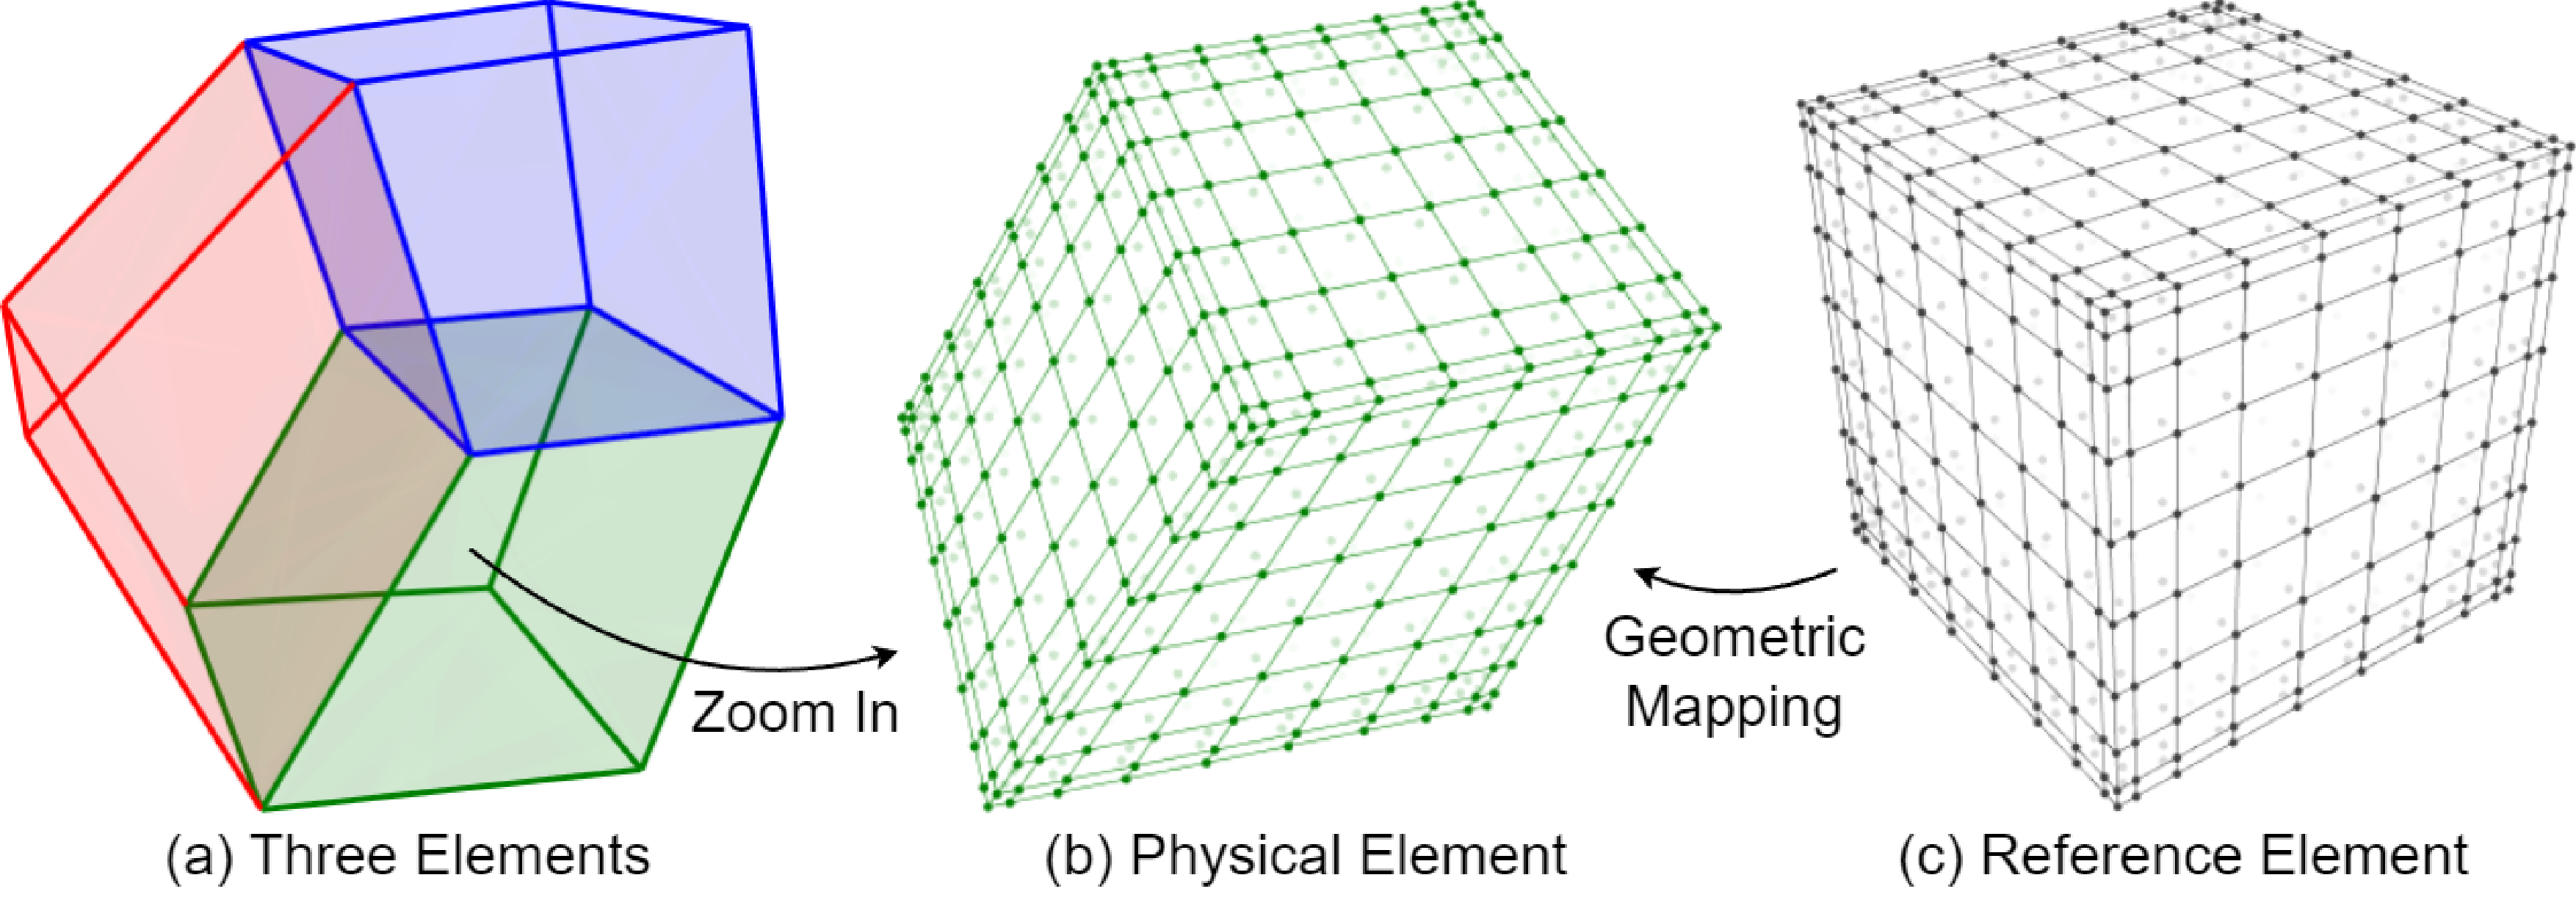
\includegraphics[width=\linewidth]{figs/3/three_elements.pdf}
    \caption{Hybrid organization of HOHS datasets. (a) Globally, physical elements exhibit irregular inter-element connectivity. (b) Locally, each physical element contains a deformed tensor-product grid of data points. (c) These physical elements are obtained by geometrically mapping a common fixed reference element.}
    \label{fig:characterizing-hohs}
\end{figure}

At a local scale, the HOHS data exhibit a markedly different structure. Within each element, the number of data points is fixed and identical for all elements. These points are arranged in a deformed tensor-product layout, typically forming an $n \times n \times n$ grid. Figure~\ref{fig:characterizing-hohs}(b) illustrates this structure using the green element in Figure~\ref{fig:characterizing-hohs}(a) as an example, which contains $10 \times 10 \times 10$ data points. For visual clarity, the figure highlights the data points close to the three visible faces of the element.

For a given element shape, all elements are derived from a common reference element with a canonical shape. Inside the reference element, the coordinates of data points in each dimension take values from a fixed set. In practice, most solvers adopt sets associated with specific high-order polynomial bases due to considerations such as numerical stability, accuracy, and quadrature compatibility. Among these, Gauss-Lobatto-Legendre (GLL) points are particularly common because they enable accurate numerical quadrature for high-order polynomial integrands while including the element boundaries. Figure~\ref{fig:characterizing-hohs}(c) illustrates the GLL node distribution in the reference element. The data points shown in Figure~\ref{fig:characterizing-hohs}(b) can be viewed as a physical-space mapping of this reference element. Although alternative sets may be supported, our examination of several representative frameworks shows that GLL points are consistently used under default settings.

During simulation, data values are first computed in the reference element and subsequently mapped to their corresponding locations in physical spaces. 
The deterministic element-local point distributions and data generation process are key to the compression design proposed in this work.

\subsection{Problem Formulation}

\begin{figure}[htb]
    \centering
    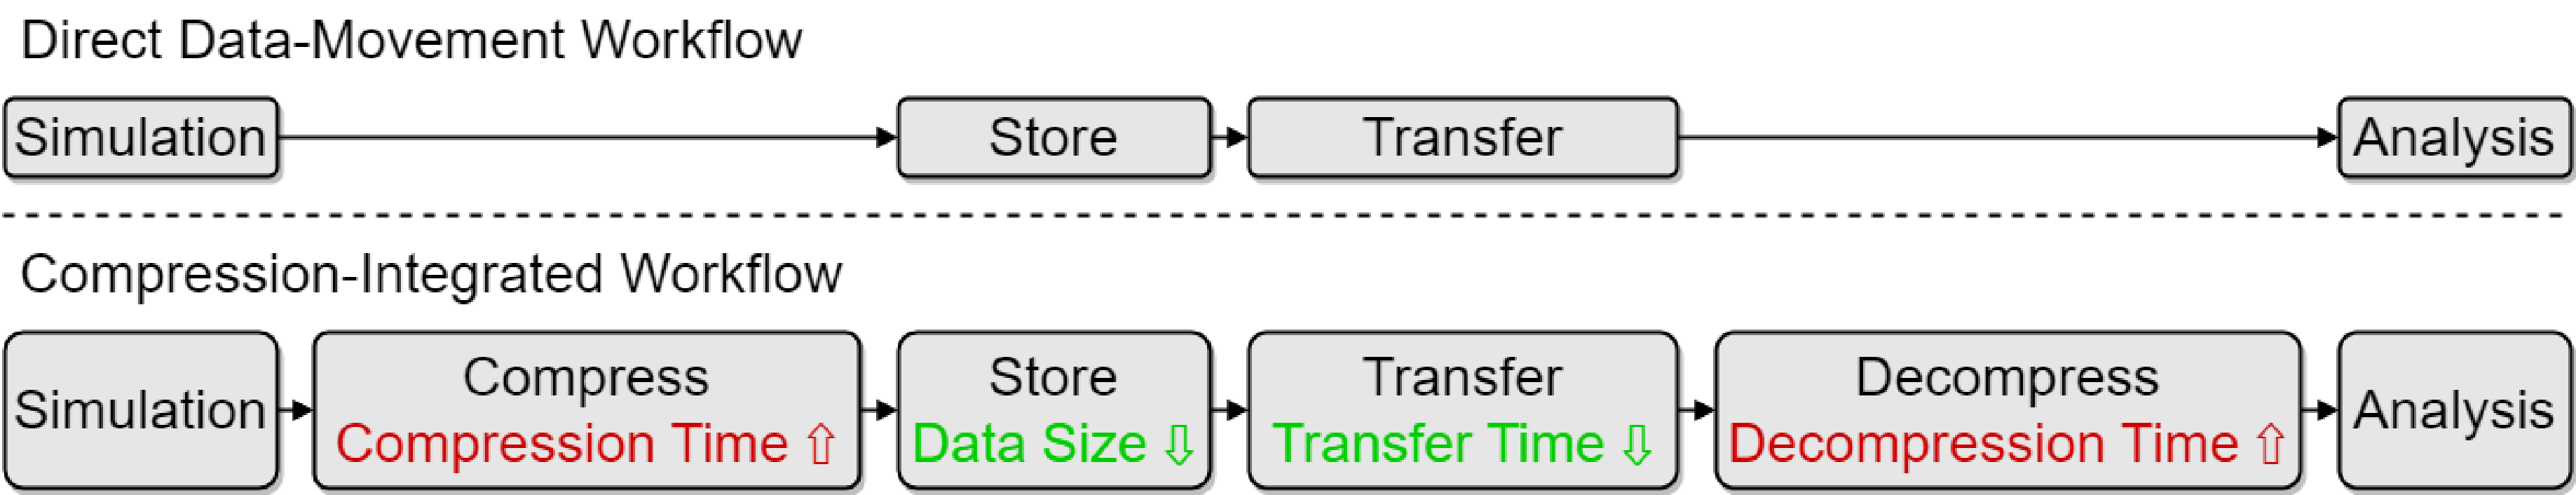
\includegraphics[width=1\linewidth]{figs/3/End to End.pdf}
    \caption{Compression-Integrated Data-Management Workflow}
    \label{fig:end-to-end}
\end{figure}

In this work, we use compressors to improve HOHS data management, but their effectiveness is non-trivial and must be evaluated from multiple perspectives. As illustrated in Figure~\ref{fig:end-to-end}, compression often reduces storage footprint and transfer volume, but it also introduces compression and decompression overhead. Ideally, a data-reduction method would provide a high compression ratio with negligible computational overhead, thereby reducing end-to-end data-movement time. In practice, however, higher compression ratios often require more sophisticated algorithms and longer computation time.

In this paper, we evaluate HOHS data reduction along two primary dimensions: the storage footprint of the reduced data under comparable data quality, and the overall end-to-end time required for compression, data movement, and decompression. These dimensions are assessed through three evaluation metrics.
\begin{itemize}
    \item \textbf{\textit{Data Quality}} characterizes the fidelity of reconstructed simulation data. It can be quantified using numerical metrics such as the prescribed upper error bound and peak signal-to-noise ratio (\textit{PSNR}). While these metrics provide convenient numerical measures, domain scientists often place greater emphasis on the \textit{visual fidelity} of simulation results. Accordingly, we also assess reconstruction quality through visualization-based evaluations, which are presented in Section~\ref{sec:performance evaluation:visualization}.
    \item \textbf{\textit{Storage Reduction}} measures the reduced storage footprint achieved under a given data-quality constraint. We report this using either the \textit{compression ratio} or the \textit{bit rate}. The compression ratio is defined as the size of the original data divided by the size of the compressed representation, whereas the bit rate denotes the average number of bits required per data value after reduction. These two metrics provide equivalent views of storage efficiency.
    \item \textbf{\textit{End-to-End Runtime}} measures the net practical cost of using data reduction in realistic data-movement workflows. We evaluate the total time required for compression, network transmission of the reduced data via Globus, and decompression.
\end{itemize}

To make such compression-based data reduction suitable for HOHS data management, the method should satisfy two key requirements.
\begin{itemize}
    \item \textbf{\textit{Field Independence}}: Different physical fields may have different accuracy requirements and downstream analysis semantics. The method should therefore support independent reduction of each field, allowing users to specify field-level quality constraints while avoiding unnecessary coupling across heterogeneous variables.
    \item \textbf{\textit{Error-bound Guarantee}}: The reduction process must satisfy a pointwise error-bound guarantee. Specifically, given a user-specified error bound $\varepsilon$, each reconstructed value must differ from its corresponding original value by no more than $\varepsilon$, under either an absolute or relative error criterion. This guarantee is essential for maintaining the fidelity of downstream scientific analysis.
\end{itemize}
\section{Design Overview}\label{sec:design overview}

This section provides a high-level overview of our HOHS data-reduction framework. We present the overall framework in Figure~\ref{fig:overview}, followed by a summary of the SZ-based pipeline that serves as the foundation of SZ3-HOHS and MRCZ. We then introduce the preprocessing steps and design considerations for HOHS data that are applied across all compressors.

\begin{figure}[htb]
    \centering
    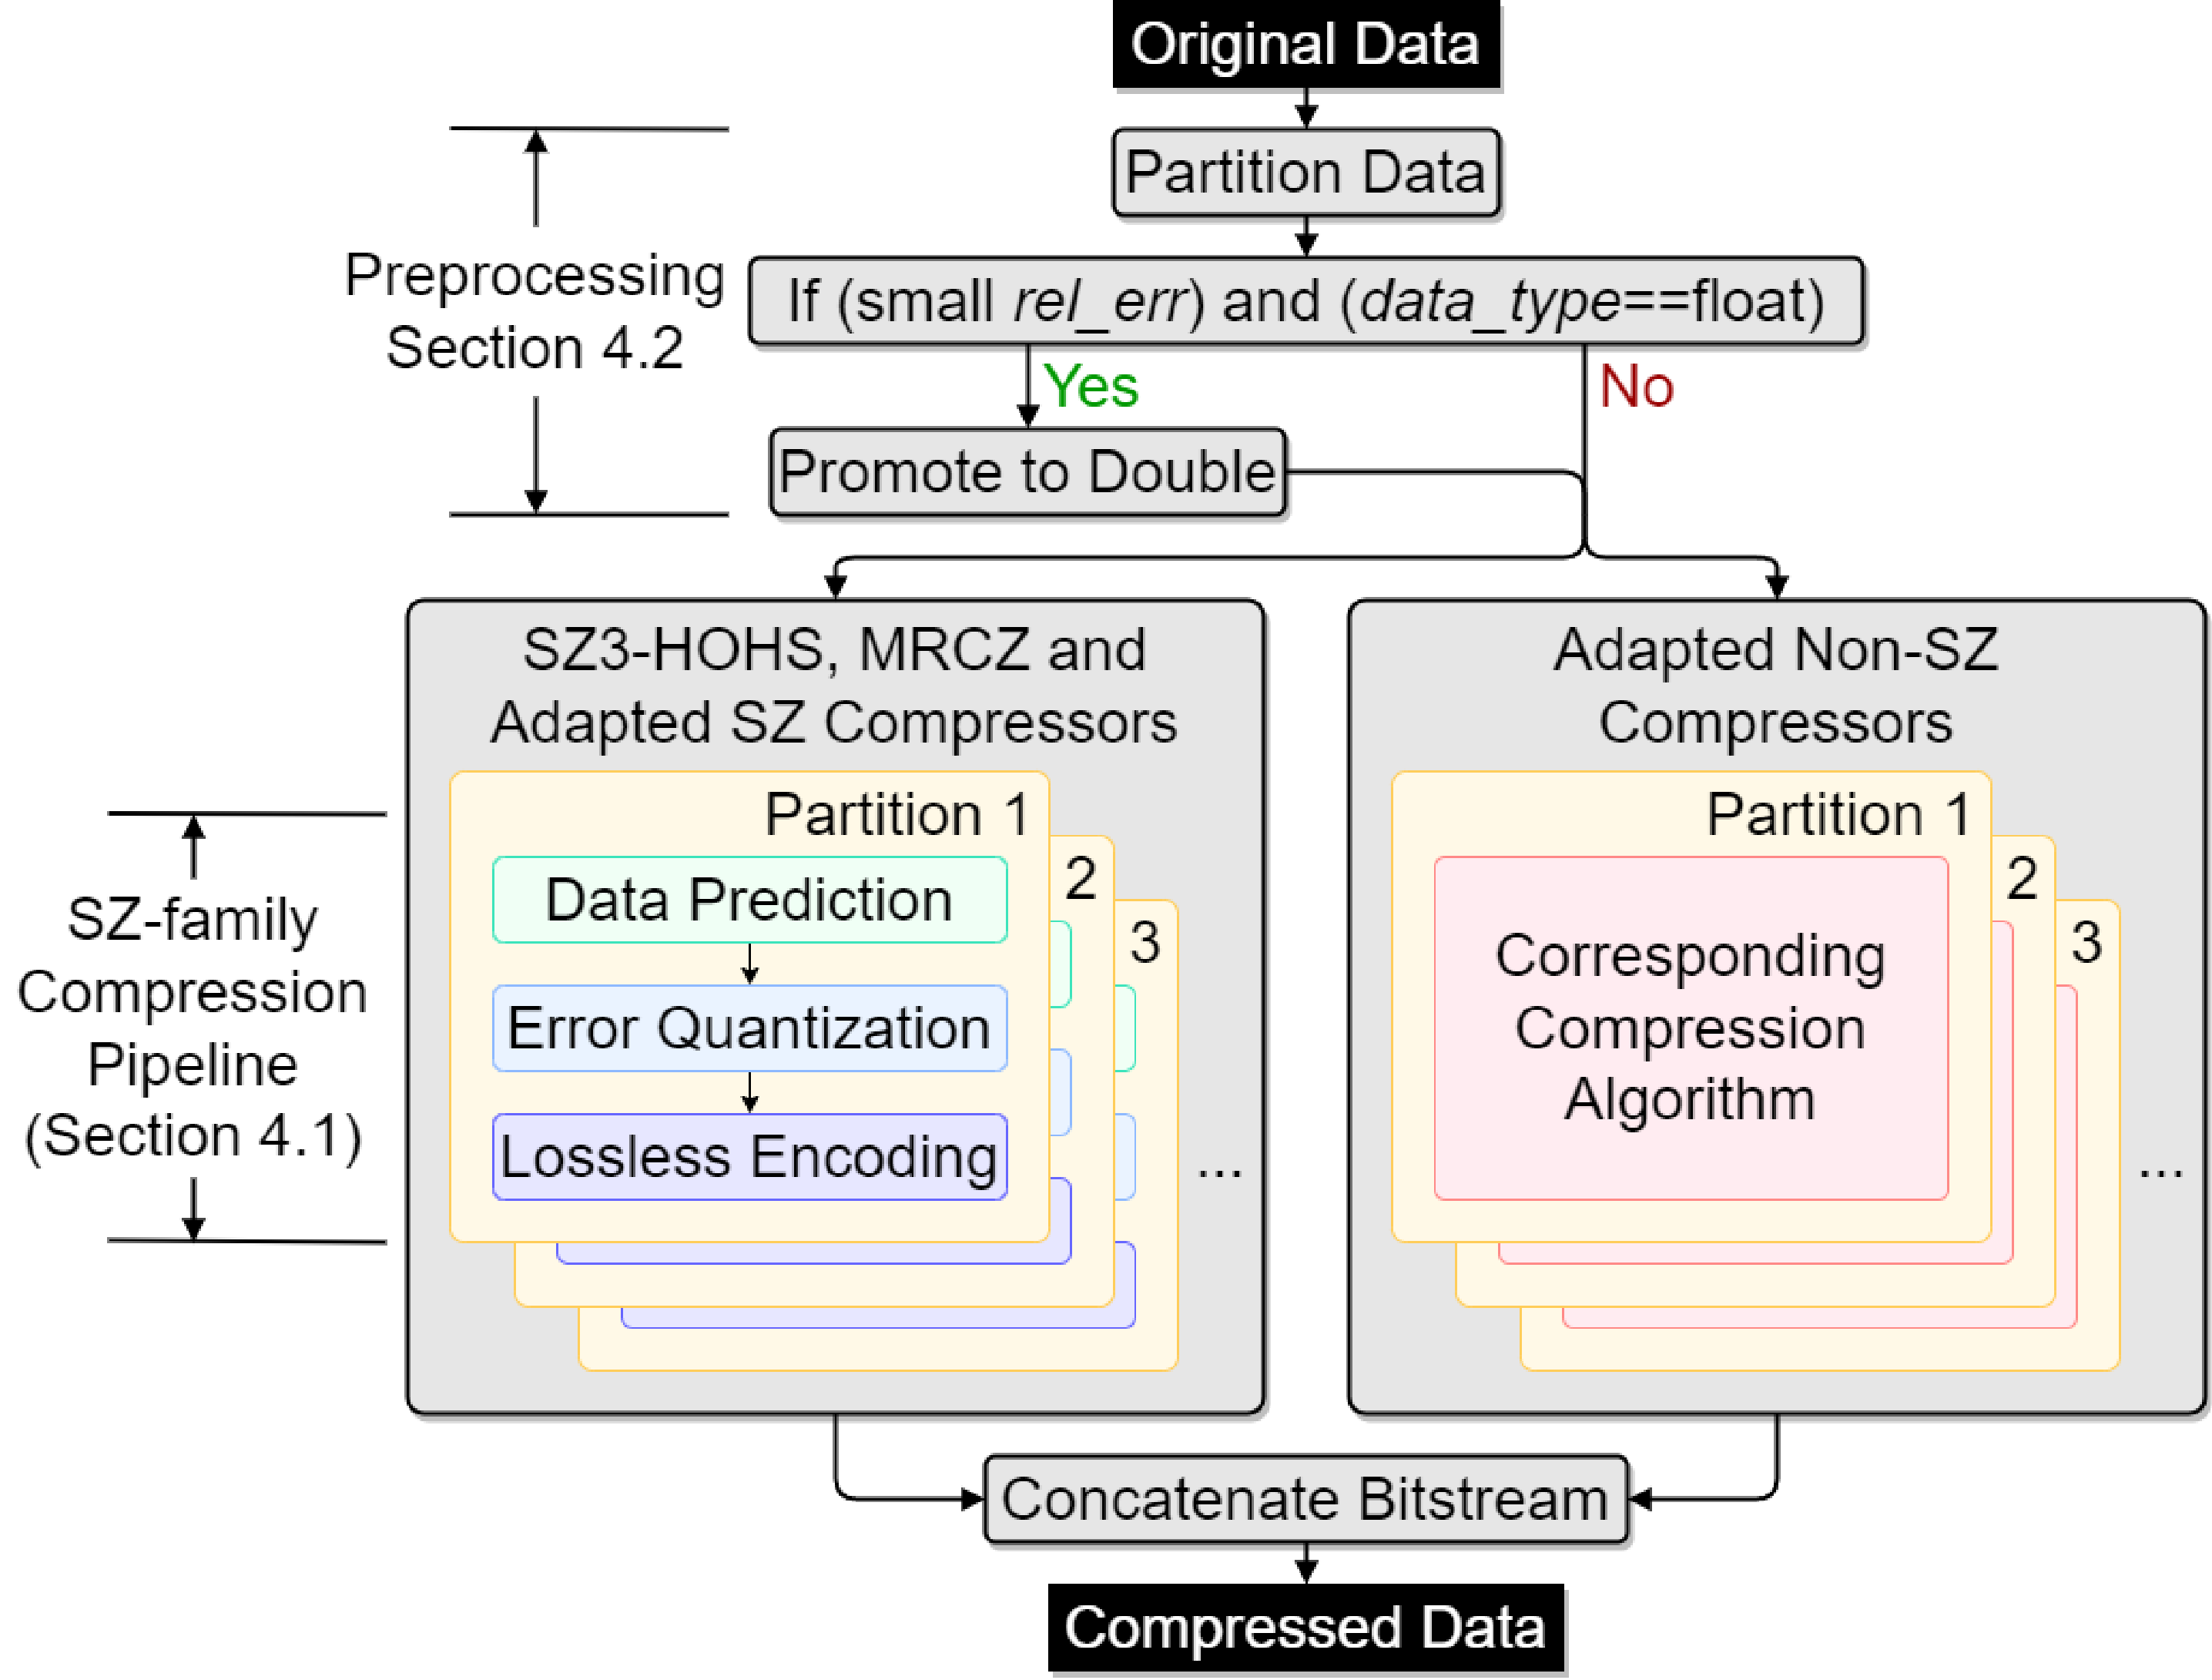
\includegraphics[width=\linewidth]{figs/4/Overall Framework.pdf}
    \caption{Overall Framework for HOHS Data Reduction}
    \label{fig:overview}
\end{figure}

\subsection{SZ-family Compression Pipeline}\label{sec:design overview:family}

Both SZ3-HOHS and MRCZ adopt the standard SZ-family compression pipeline~\cite{di2016fast,tao2017significantly,liang2018error,zhao2021optimizing,liang2022sz3}. As shown in Figure~\ref{fig:overview}, this pipeline follows a classic prediction-based model consisting of three main stages: \textit{data prediction}, \textit{error-bounded quantization} of prediction residuals, and \textit{lossless encoding} of the resulting quantization symbols. During prediction, each data value is estimated using a predictor constructed from available reference information. The difference between the original and predicted values is then quantized under a user-specified error bound, ensuring that the reconstructed data satisfy the prescribed pointwise error constraint. Finally, the resulting quantization symbols are encoded losslessly, typically using a combination of Huffman coding and Zstandard~\cite{zstd}.

Prediction accuracy is critical to the effectiveness of SZ-family compressors. More accurate prediction generally produces smaller residuals and causes the corresponding quantization symbols to concentrate around zero. The resulting lower-entropy distribution can be encoded more efficiently and therefore generally leads to a higher compression ratio. Existing SZ compressors employ different prediction strategies. SZ1~\cite{di2016fast}, SZ3~\cite{liang2022sz3,zhao2021optimizing}, and QoZ2.0~\cite{liu2024high} use iterative schemes, in which previously reconstructed values are used to predict subsequent data points. In contrast, SZ2~\cite{tao2017significantly} adopts a non-iterative, block-based regression approach that generates model coefficients, which are quantized and stored as auxiliary information for reconstruction.

In addition to their statistical distribution, local regularity and repeated patterns in the quantization-symbol sequence can further improve the effectiveness of subsequent lossless compression. Recent variants, including SZ3~\cite{liang2022sz3,zhao2021optimizing} and QoZ2.0~\cite{liu2024high}, incorporate optimizations that improve such regularity.

Within this common pipeline, SZ3-HOHS adopts an iterative prediction strategy consistent with SZ3-style designs~\cite{liang2022sz3,zhao2021optimizing}, whereas MRCZ employs a model-based prediction strategy that is conceptually closer to the non-iterative approach used in SZ2~\cite{tao2017significantly}. Our primary contribution is the development of prediction methods tailored to the structural characteristics of HOHS data.

\subsection{General Preprocessing for HOHS Data}

Two general preprocessing steps are applied to HOHS data for our developed methods and other methods to be evaluated in this paper. First, spectral elements in HOHS data are grouped into multiple partitions based on their ordering within each field, and each partition is processed independently by a separate OpenMP thread. This element-centric organization enables straightforward parallelization without introducing inter-thread dependencies, while also preserving contiguous memory access within each thread. Second, when the input data are stored in single-precision floating-point format, and very small relative error bounds are specified, numerical precision may become insufficient due to amplified round-off errors. In such cases, the input data are conditionally promoted to double precision.

\subsection{Element-local Design Considerations}

In our design, we restrict prediction to be element-local and do not explicitly exploit correlations across neighboring elements. This choice is motivated by three considerations.

\begin{enumerate}
\item \textit{Irregular Connectivity}: Elements in HOHS data are connected in an unstructured manner, and each element is associated with its own local coordinate system. Exploiting cross-element correlations would require identifying adjacent elements sharing a common face and aligning their orientations, which introduces computational complexity and non-trivial overhead.
\item \textit{Prediction Accuracy}: Although neighboring elements may exhibit physical correlations, exploiting them does not necessarily improve prediction accuracy. In our experiments, extending prediction across element boundaries often reduces prediction accuracy compared with element-local prediction. A detailed evaluation is provided in Section~\ref{sec:SZ3-HOHS:cross_element}.
\item \textit{Transform Locality}: The model-based transform used in MRCZ operates on data within individual elements, where the data naturally form tensor-product structures, which are not preserved across element boundaries, making it difficult to extend the transform consistently.
\end{enumerate}


\section{Interpolation-Based Compression: SZ3-HOHS}\label{sec:SZ3-HOHS}

In this section, we describe the interpolation-based prediction used in SZ3-HOHS. We first review the interpolation strategy in SZ3 as background, then introduce our modifications to adapt it to the non-uniform layout of HOHS data. Finally, we examine the effectiveness of cross-element prediction.

\subsection{Interpolation Prediction in SZ3}\label{sec:SZ3-HOHS:sz3 interpolation}

SZ3 employs a multi-dimensional prediction scheme, where the prediction of each data point is carried out along a particular dimension that can change from point to point. The compressor provides both linear and cubic interpolation predictors. In SZ3-HOHS, we focus on the linear interpolation predictor, which estimates each target data point using two reference points along a given dimension, due to its low computational cost.

For the linear interpolation in SZ3, as shown in Figure~\ref{fig:sz3 interpolation}, each data point is predicted using two neighboring values located at equal distances on opposite sides of the target point. The predicted value is computed as the arithmetic mean of these two references. This operation can be interpreted as fitting a linear function through the reference points and evaluating it at the target location. Owing to the symmetric placement of the neighbors, the prediction naturally reduces to their simple average.
Another situation involving two reference points arises as a boundary case of cubic interpolation, as illustrated in Figure~\ref{fig:sz3 interpolation}. Both reference points lie on the same side of the prediction target. In this case, the fitted model degenerates to a linear function defined by asymmetric reference positions, and the prediction becomes a weighted average rather than a simple mean.

\begin{figure}[htb]
    \centering
    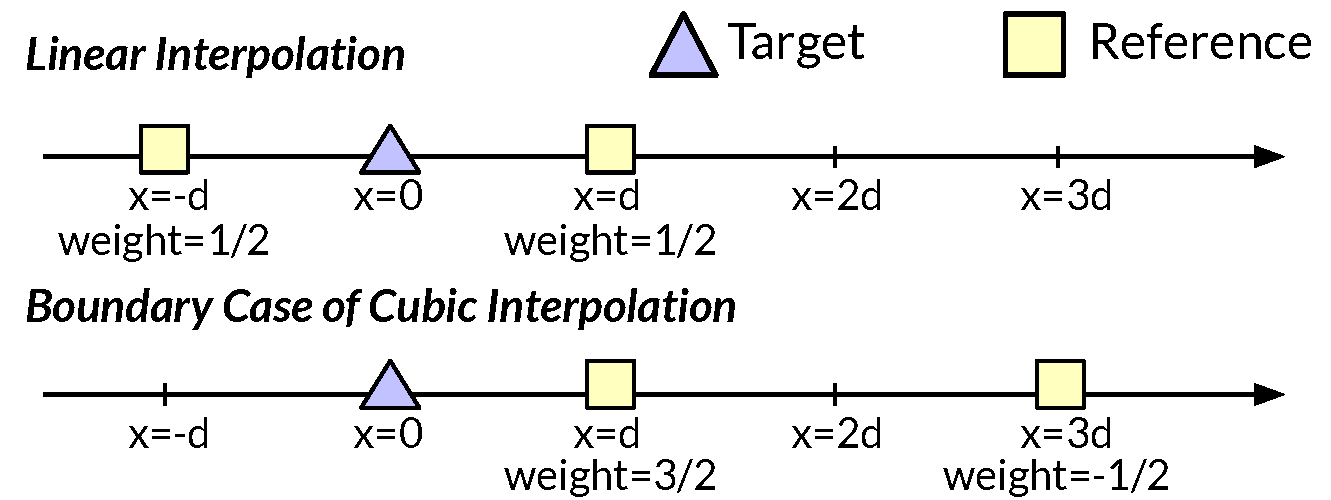
\includegraphics[width=0.9\linewidth]{figs/2-two-types-interpolation-in-sz3.pdf}
    \caption{Two Types of Interpolation in SZ3}
    \label{fig:sz3 interpolation}
\end{figure}

\subsection{Interpolation Prediction in SZ3-HOHS}

SZ3-HOHS extends the interpolation-based prediction strategy of SZ3 to accommodate the non-uniform spacing of data points in HOHS datasets. This adaptation involves two changes: distance-aware interpolation weights and a modified prediction order.

\begin{figure}[htb]
    \centering
    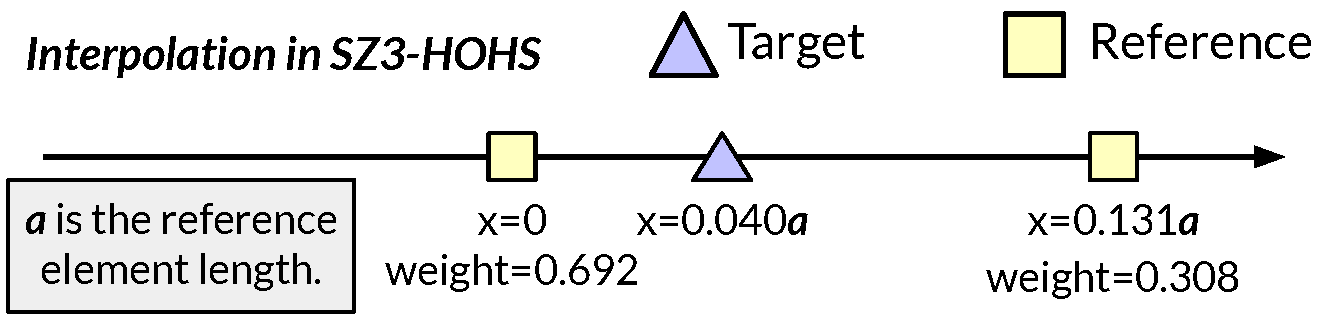
\includegraphics[width=0.9\linewidth]{figs/3-interpolation-in-hohs.pdf}
    \caption{Interpolation Method in SZ3-HOHS}
    \label{fig:sz3-hohs-interpolation}
\end{figure}

\begin{enumerate}
\item \textit{Distance-aware Interpolation Weights}: SZ3-HOHS adjusts the interpolation weights according to the relative physical distances between the prediction target and its reference points. Figure~\ref{fig:sz3-hohs-interpolation} shows an example of such non-uniform spacing. In this example, the distances from the target point to the closer and farther reference points are $0.040a$ and $0.091a$, respectively, corresponding to a distance ratio of approximately $1{:}2.26$, where $a$ denotes the length of the reference element. Accordingly, the closer reference point receives a larger interpolation weight, with the two weights being $0.692$ and $0.308$, respectively, corresponding to a weight ratio of approximately $2.26{:}1$.
\item \textit{Modified Prediction Order}: In SZ3, linear interpolation always chooses the data point located at the midpoint of the two reference points as the prediction target, where the notion of ``middle'' is well defined in both physical space and array index due to the structured layout of the data. In contrast, SZ3-HOHS selects the unpredicted data point closest to the physical center of the two reference points. This choice avoids overly extreme interpolation weights for the reference points, such as values close to 0 or 1. From a statistical perspective, it helps mitigate the propagation of compression errors from the reference points to the target.
\end{enumerate}

Another key observation of SZ3-HOHS is that, although physical spacing may vary across elements, the logical organization of data points within each element is fixed by the reference element and the associated GLL points~\cite{Isoparametric-Mapping}. Consequently, both the prediction order and the interpolation weights can be determined entirely from the reference element prior to compression. These prediction parameters are precomputed once and reused across all elements with the same polynomial order, eliminating the need for runtime distance calculations and ensuring negligible overhead.

In addition, SZ3-HOHS exhibits a slight performance advantage over SZ3 with respect to memory access behavior. When applied to large regular tensor datasets, SZ3 may involve long-range prediction accesses that can incur cache misses. In HOHS datasets, however, individual elements are typically small, often no larger than $10 \times 10 \times 10$, allowing SZ3-HOHS to operate primarily on cache-resident, element-local data.

\subsection{Evaluation of Cross-Element Prediction}\label{sec:SZ3-HOHS:cross_element}

\begin{figure}[htb]
    \centering
    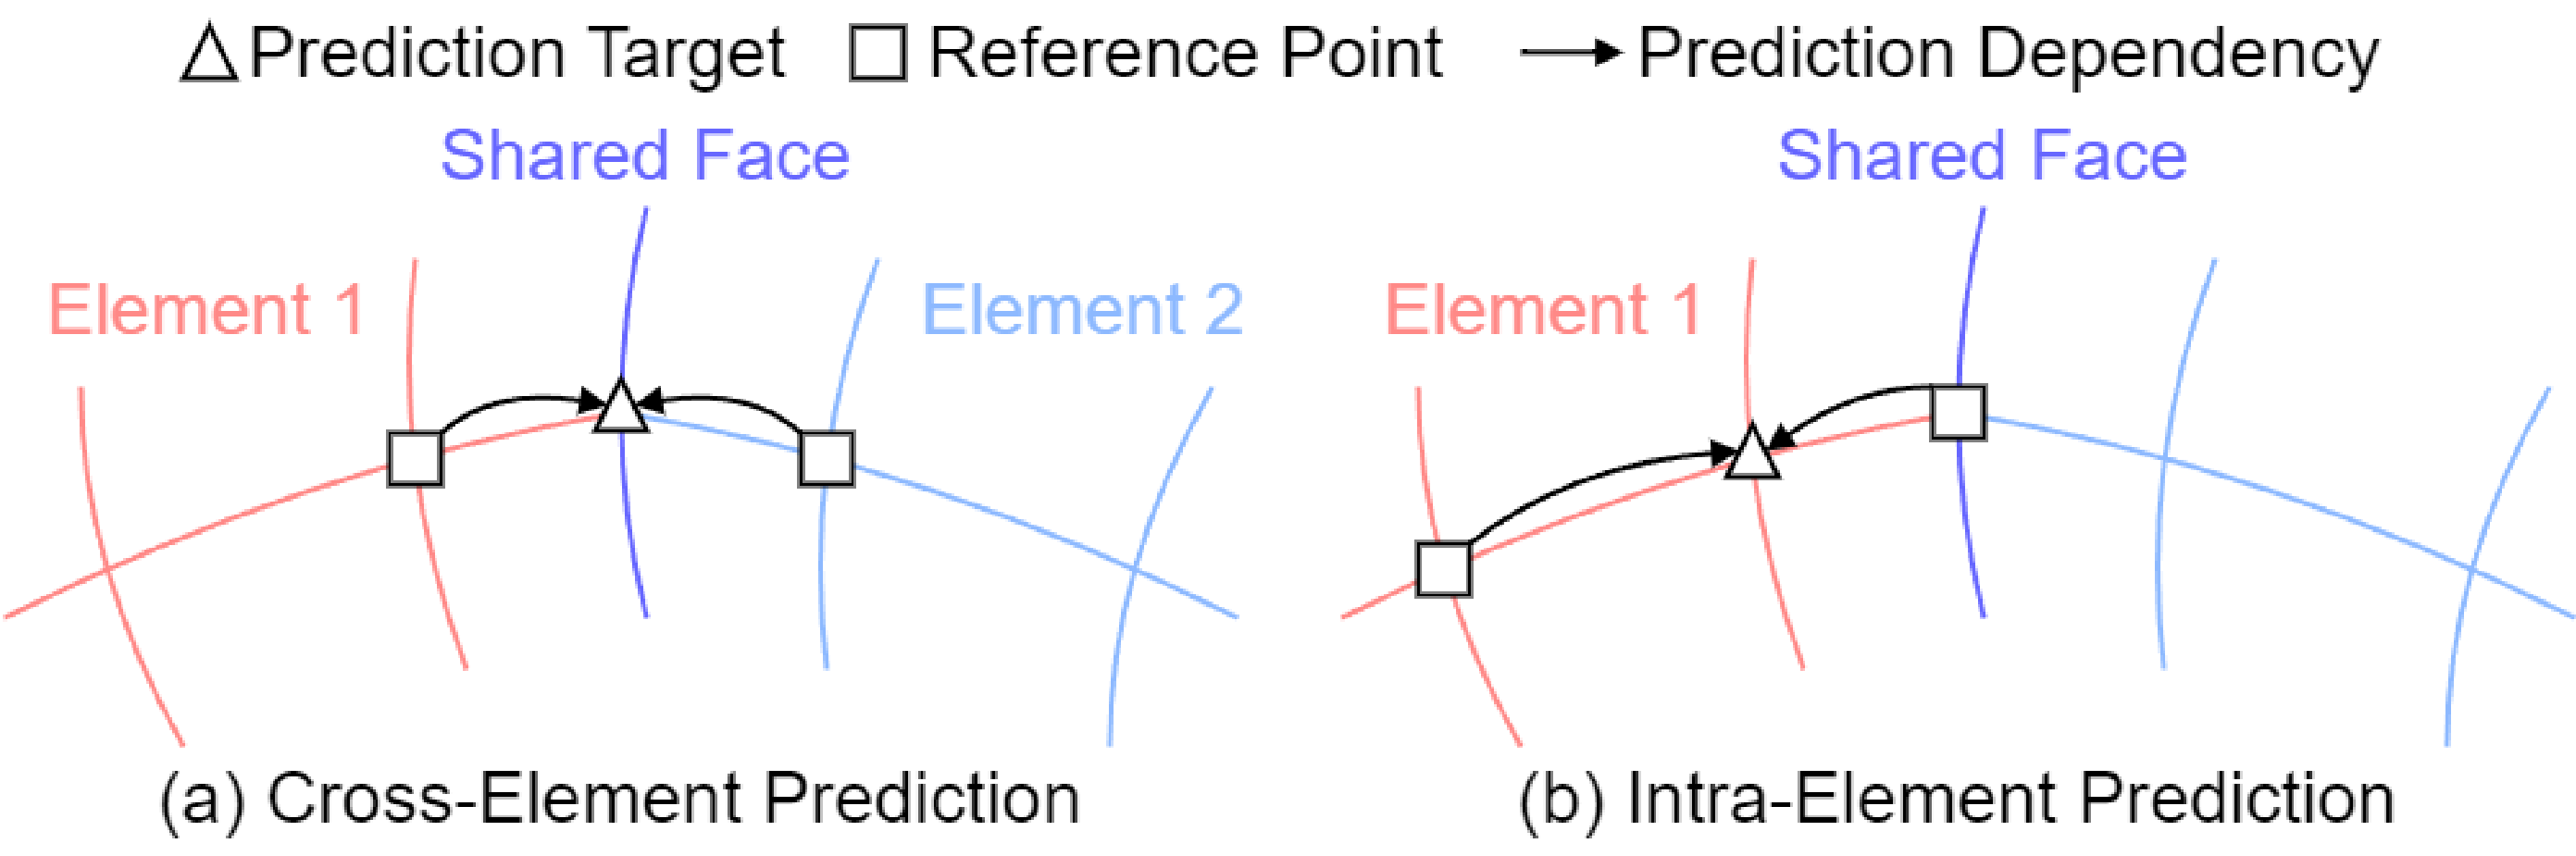
\includegraphics[width=1\linewidth]{figs/5/cross-element.pdf}
    \caption{Illustration of the Point Configurations Used in Cross-Element and Intra-Element Prediction}
    \label{fig:cross-element}
\end{figure}

We further explain the rationale for using intra-element prediction instead of cross-element prediction in SZ3-HOHS. In principle, cross-element prediction may benefit from the dense sampling near element boundaries. Since the physical distance between points across a shared face is small, their values may be more similar than those of neighboring points closer to the element interior, which can improve prediction accuracy. However, the reference points used in cross-element prediction are generally not collinear with the prediction target in physical space, which can reduce the effectiveness of linear interpolation. By contrast, the target and reference points used for intra-element prediction are collinear in the reference element and remain nearly collinear in physical space, with only minor distortion introduced by the element mapping. These competing effects make it unclear a priori which strategy provides more accurate predictions. We therefore perform an empirical comparison of cross-element and intra-element prediction.

We conduct experiments on the NekRS dataset~\cite{fischer2022nekrs} with an element size of $8\times8\times8$ (Dataset 4 in Table~\ref{tab:datasets}). We randomly sample a subset of elements, identify their neighboring elements, and align the neighboring elements to ensure consistent face orientations. For cross-element prediction, each point on the shared face is treated as a prediction target, and one neighboring interior grid point from each of the two adjacent elements is used as a reference for weighted linear interpolation. For comparison, the intra-element scheme predicts the same target using two reference points from the same element, both selected along the grid line extending from the shared face into the element interior. In both cases, prediction accuracy is quantified using mean squared error (MSE).

% \begin{table}[h]
%     \caption{MSE between cross-element and intra-element predictions across five faces of element 1940839.}
%     \label{tab:cross-element mse}
%     \centering
%     \begin{tabular}{c|cc}\toprule
%         \textbf{Adjacent Element} & \textbf{Cross-Element MSE} & \textbf{Intra-Element MSE} \\\midrule
        
%         1940803 & 2.049e-09 & 1.842e-08 \\
%         1940840 & 6.993e-04 & 1.146e-05\\
%         1940827 & 2.695e-07 & 3.909e-07\\
%         1940833 & 4.341e-08 & 2.526e-07\\
%         1940849 & 7.868e-06 & 1.031e-06\\\bottomrule
%     \end{tabular}
% \end{table}

\begin{table}[h]
    \caption{Comparison of Cross-Element and Intra-Element Prediction MSEs of a Representative Element}
    \label{tab:cross-element mse}
    \centering
    \begin{tabular}{c|cc}\toprule
        \textbf{Face Index} & \textbf{Cross-Element MSE} & \textbf{Intra-Element MSE} \\\midrule
        1 & 2.049e-09 & 1.842e-08 \\
        2 & 6.993e-04 & 1.146e-05\\
        3 & 2.695e-07 & 3.909e-07\\
        4 & 4.341e-08 & 2.526e-07\\
        5 & 7.868e-06 & 1.031e-06\\\bottomrule
    \end{tabular}
\end{table}

Table~\ref{tab:cross-element mse} presents the results for a representative element with five faces that have adjacent elements. Its remaining face has no identifiable adjacent element and is therefore excluded from the comparison. Additional tests show that either cross-element or intra-element prediction may achieve lower MSE on an individual face, while their average MSEs over a large number of faces are comparable. Thus, cross-element prediction provides no consistent accuracy advantage to justify the additional overhead of connectivity identification and orientation alignment. We therefore adopt intra-element prediction in SZ3-HOHS.
\section{Representation-Based Compression: MRCZ}\label{sec:mrcz}

In this section, we first analyze the compressor introduced in Section~\ref{sec:related work:prior work} in detail. Building on this foundation, we progressively analyze and optimize its design, and ultimately develop a new model-representation-based compressor, MRCZ.

\subsection{Revisiting DLT for HOHS Data Compression}

In Section~\ref{sec:related work:prior work}, we introduced a compressor~\cite{marin2016spectral} for HOHS data generated by Nek5000, which applies discrete Legendre transforms (DLT) on elements defined on GLL nodes. A key observation motivating this approach is that the transformed coefficients tend to be significantly more concentrated than the original data values.
To verify this, we take the 5th NekRS~\cite{fischer2022nekrs} dataset in Table~\ref{tab:datasets} and report the value-frequency distribution.

\begin{figure}[htb]
    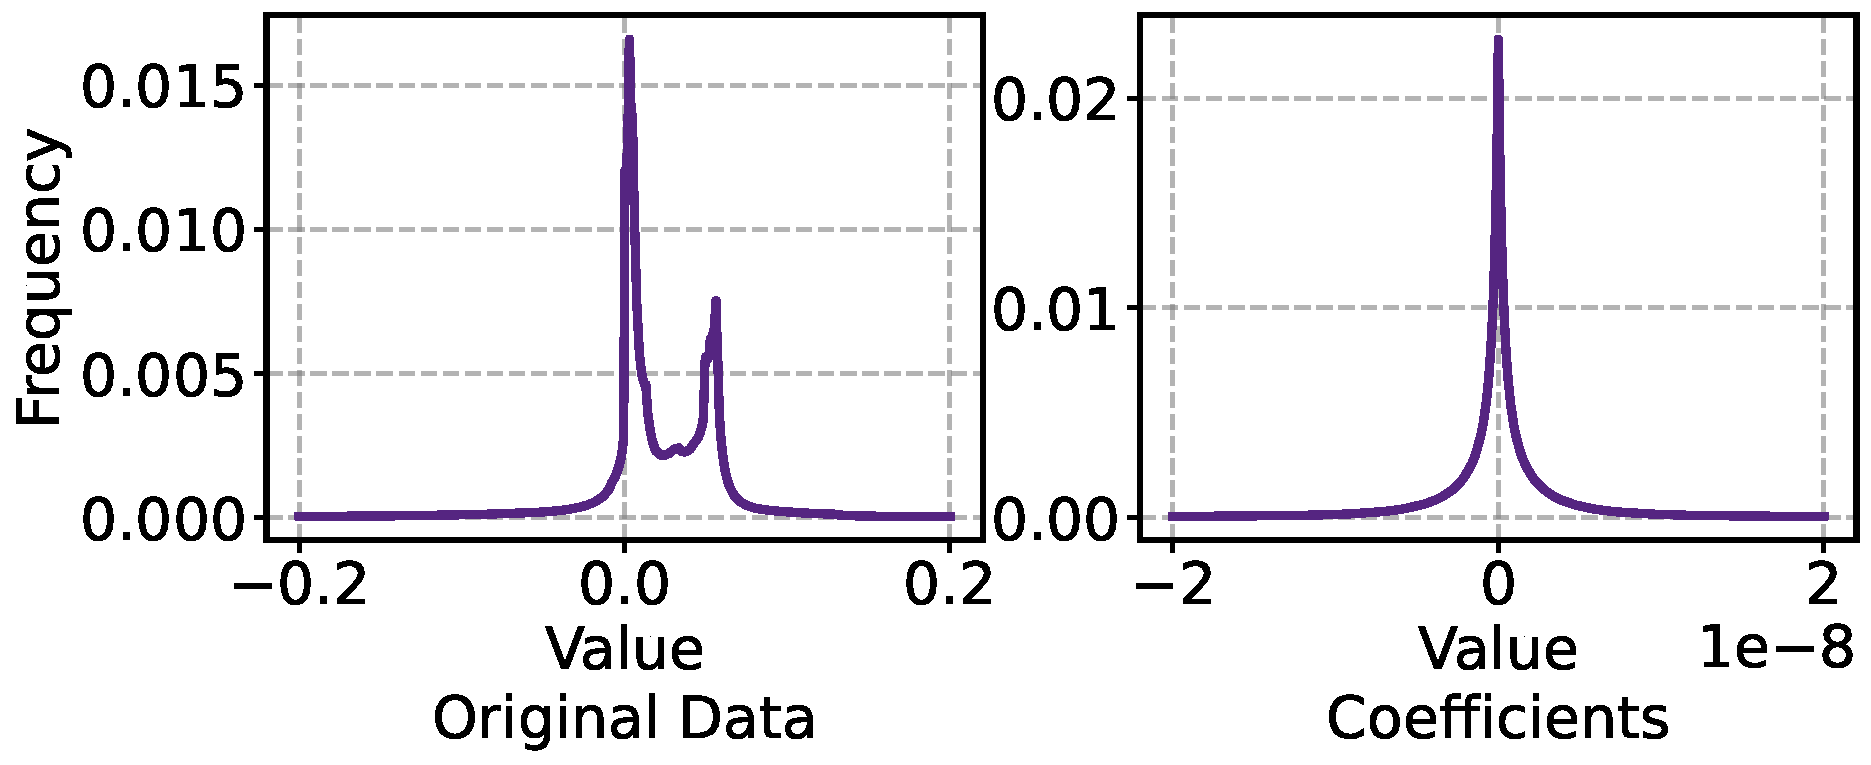
\includegraphics[width=0.8\linewidth]{figs/4-distribution-of-data-and-coefficients.pdf}
    \caption{Distributions of Original Data and Coefficients}
    \label{fig:dlt_distributions}
\end{figure}

Figure~\ref{fig:dlt_distributions} compares the distributions of the original data and the coefficients obtained by applying the DLT to HOHS data defined on GLL nodes. In this example, most coefficients are confined to a range approximately $10^{-7}$ times as wide as the range containing most of the original data. This strong concentration benefits the thresholding strategy used in the previously mentioned method~\cite{marin2016spectral}, which sets sufficiently small coefficients to zero. A more concentrated coefficient distribution, therefore, allows a larger fraction of coefficients to be zeroed, thereby reducing the storage footprint. Moreover, because the Legendre basis is orthogonal under the GLL quadrature-weighted inner product, errors introduced by coefficient thresholding are not strongly amplified during the inverse transform. Thus, discarding coefficients of sufficiently small magnitude generally leads to limited reconstruction error.

However, the reconstruction error introduced by the previously discussed thresholding method is only indirectly controlled and does not necessarily satisfy a user-specified pointwise error bound. In contrast, as described in Section~\ref{sec:design overview:family}, the SZ framework enforces the prescribed error bound independently of the specific prediction strategy, whether it is interpolation-based or transform-based. Therefore, strict orthogonality of the transform is not essential for error control. As long as the transform is invertible and numerically stable, its primary role is to produce coefficients that are more compressible. This observation decouples compression effectiveness from the mathematical properties of the DLT and suggests that alternative transforms, if better aligned with the data structure, may achieve stronger coefficient compaction. This motivates us to explore transformation choices beyond the DLT.

\subsection{Overview of MRCZ}

\begin{figure}[htb]
    \centering
    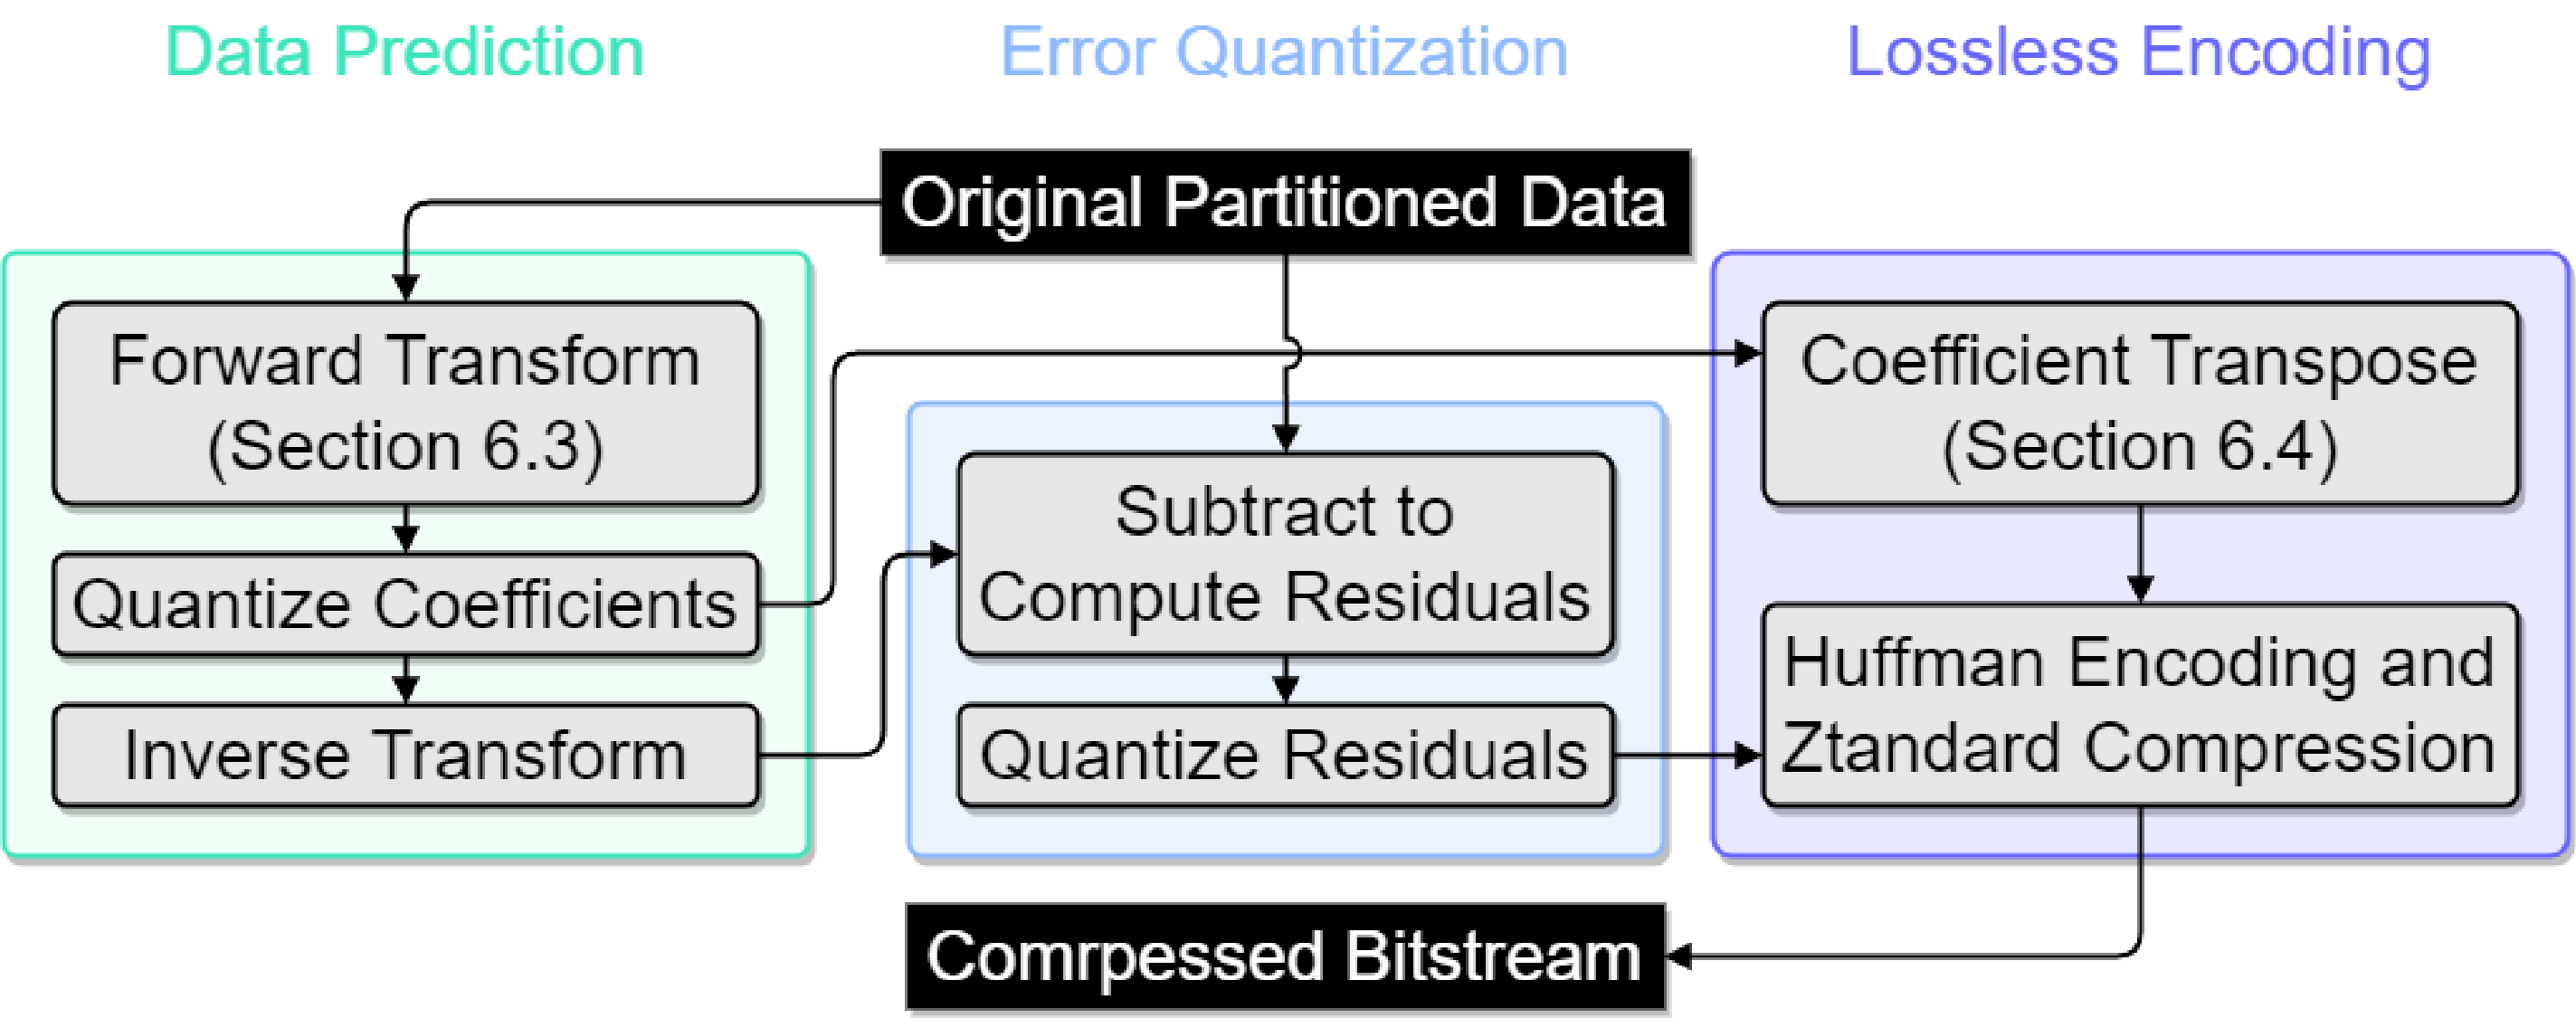
\includegraphics[width=1\linewidth]{figs/6/mrcz diagram.pdf}
    \caption{Diagram of MRCZ Compression.}
    \label{fig:mrcz_diagram}
\end{figure}

Figure~\ref{fig:mrcz_diagram} illustrates the overall workflow of MRCZ. Similar to other SZ-family compressors, MRCZ consists of three main stages: data prediction, error-bounded quantization, and lossless encoding.

During data prediction, MRCZ applies a forward transform to each element, quantizes the resulting transform coefficients using a dedicated coefficient error bound, and then performs an inverse transform on the quantized coefficients to generate approximate predictions. The residuals between the original data and these predictions are subsequently quantized under the user-specified error bound. Consequently, in addition to the quantized residuals stored by conventional SZ-family compressors, MRCZ must also store the quantized transform coefficients required to reproduce the predictions during decompression.

The residual quantization and lossless encoding stages otherwise follow the standard SZ-family pipeline described in Section~\ref{sec:design overview:family}. Before lossless encoding, MRCZ additionally transposes the quantized coefficient layout to improve its compressibility, as discussed in Section~\ref{sec:mrcz:transpose}.

\subsection{Transform and Error Bound Selection}

In addition to the choice of transform, the coefficient error bound also has a significant impact on compression performance. A smaller coefficient error bound preserves the transform coefficients more accurately, but produces more finely quantized coefficient symbols that are generally less compressible. At the same time, the resulting predictions are more accurate, leading to smaller residuals that are easier to compress. If the coefficient error bound is excessively small, the prediction error after the inverse transform may remain below the user-specified error bound for most or even all data points. In this case, the available error budget is underutilized, resulting in higher reconstruction quality than required at the cost of a lower compression ratio.

\begin{figure}[htb]
    \centering
    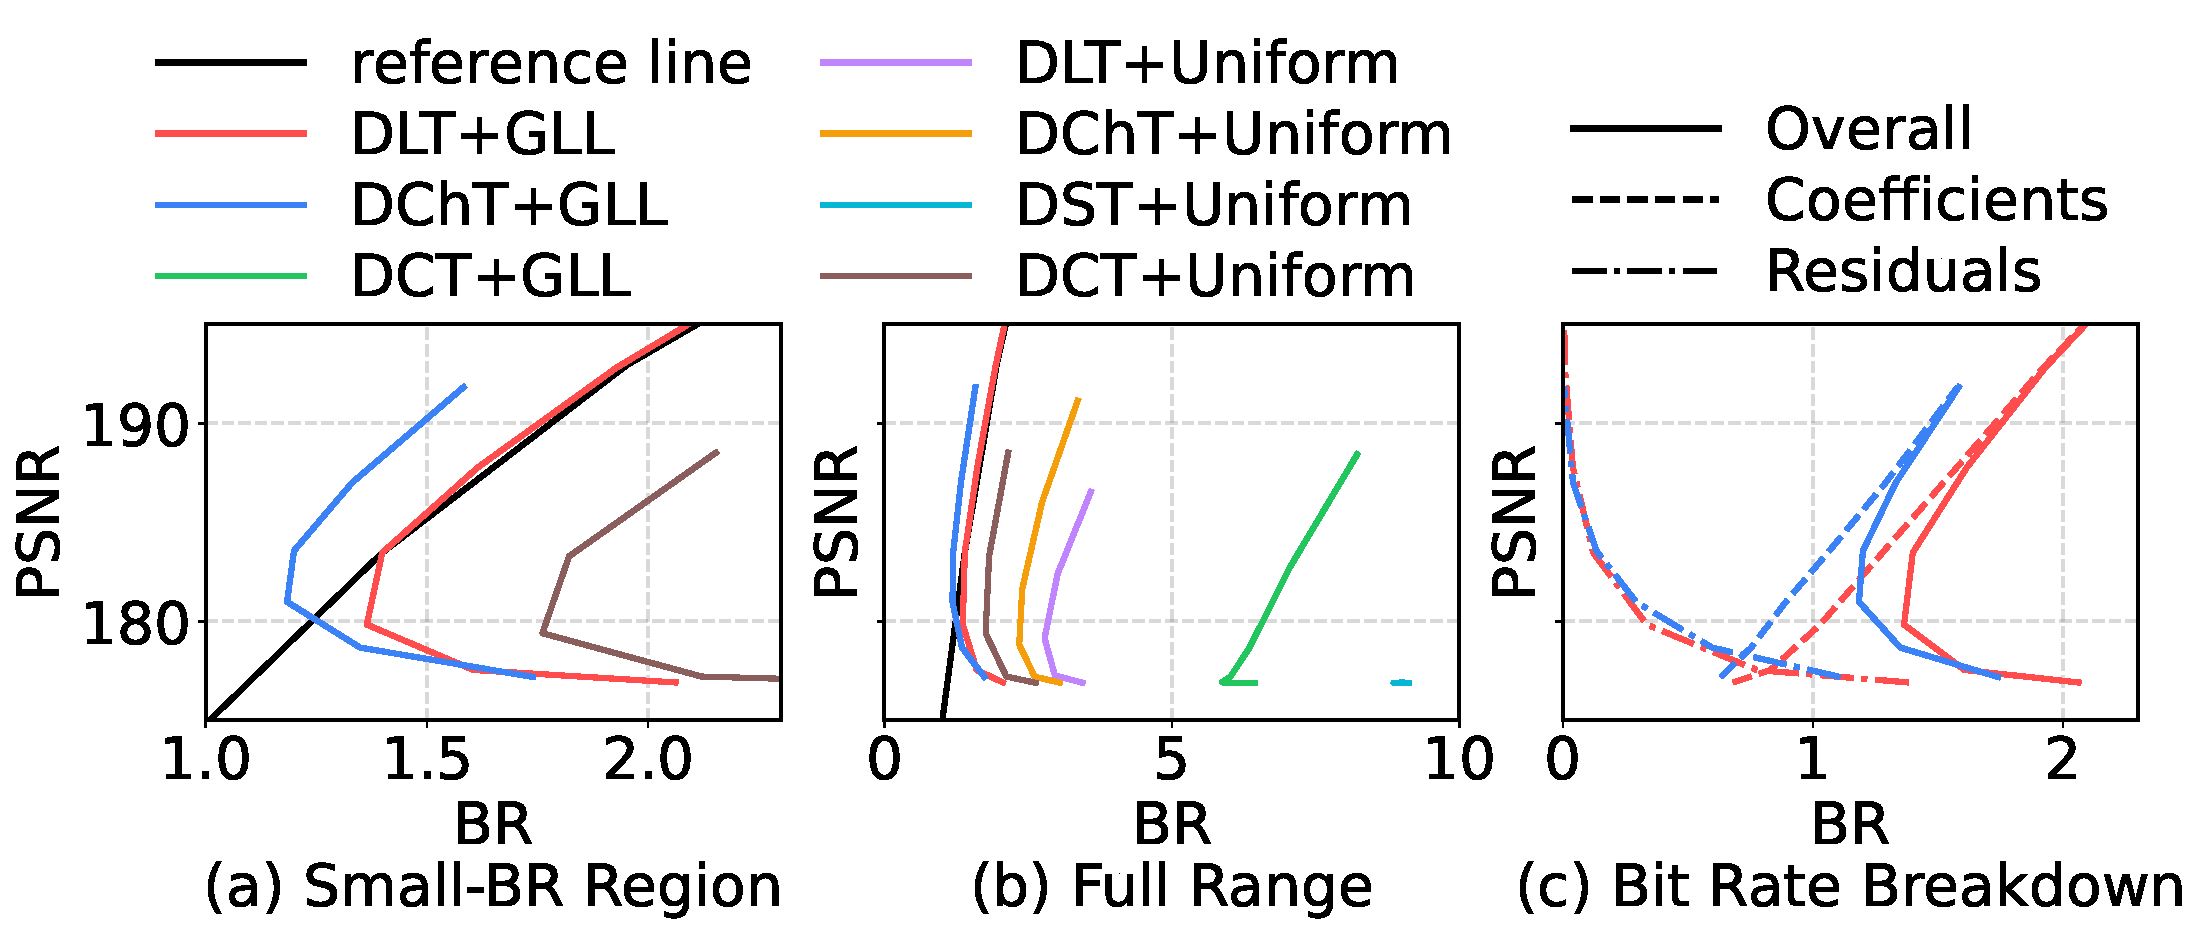
\includegraphics[width=1\linewidth]{figs/6/transform-comparison.pdf}
    \caption{Rate–Distortion Performance and Bit-Rate Breakdown of Different Transforms Across Error-Bound Configurations}
    \label{fig:transform}
\end{figure}

To study this trade-off, we use DLT as an example and define $k_{eb}=\frac{eb_{coeff}}{eb_{value}}$, where $eb_{coeff}$ is the coefficient error bound and $eb_{value}$ is the user-specified data error bound. We first fix $eb_{value}$ and vary $k_{eb}$, producing the red solid curve in Figure~\ref{fig:transform}(a). For reference, we also plot a conventional rate--distortion curve by fixing $k_{eb}$ and varying $eb_{value}$ (black solid curve). This reference curve characterizes the compressor performance under different user-specified error bounds. 

When $k_{eb}$ is too small, the red curve nearly overlaps the reference curve. In this regime, the compressor produces data with higher fidelity than required by the user, at the cost of a lower compression ratio. An appropriate value of $k_{eb}$ is therefore near the transition at which the red curve begins to deviate noticeably from the reference curve. For DLT, this transition occurs at approximately $k_{eb}=0.1$.

We next compare different transforms under the same user-specified data error bound. Figures~\ref{fig:transform}(a) and \ref{fig:transform}(b) present the rate--distortion curves for the evaluated transforms, obtained by varying $k_{eb}$, together with the black reference curve described above. We evaluate DLT, DCT, DST, and DChT using two node-location assumptions. In the figure legends, the ``GLL'' variants use the actual GLL node locations, whereas the ``Uniform'' variants treat the input values as samples on a uniformly spaced grid.

Among the evaluated transforms, DChT+GLL generally achieves the best rate--distortion performance. Portions of its curve lie to the left of the reference curve, indicating that it can achieve a lower bit rate, and equivalently a higher compression ratio, than the DLT-based reference configuration at comparable distortion levels. Overall, DChT+GLL improves the compression ratio by approximately 20\% over DLT+GLL at the same PSNR. For DChT+GLL, the corresponding transition occurs at approximately $k_{eb}=0.05$. Based on these results, we adopt DChT+GLL with $k_{eb}=0.05$ as the core transform configuration in MRCZ and refer to it simply as DChT hereafter.

To better understand the source of the performance difference between DChT and DLT, we separately compress the transform coefficients and the residuals produced by each transform. Figure~\ref{fig:transform}(c) shows the resulting rate--distortion curves for DChT and DLT on GLL nodes. The residual curves of the two transforms nearly overlap, indicating that their residuals have similar compressibility. In contrast, the coefficient curve of DChT lies consistently to the left of that of DLT, showing that the coefficients produced by DChT can be compressed at a lower bit rate for a comparable distortion level. Therefore, the overall rate--distortion advantage of DChT primarily comes from the improved compressibility of its transform coefficients rather than from differences in the residuals.

\subsection{Improving Local Regularity for Lossless Encoding}\label{sec:mrcz:transpose}

We further investigate whether the quantized transform coefficients can be made more compressible by improving their local regularity before lossless encoding. A related idea is used in QoZ2.0~\cite{liu2024high}, which applies lightweight spatial blocking based on the observation that neighboring data points often exhibit similar prediction errors. Such regularity may arise because higher-order information not fully captured by interpolation can still exhibit local spatial continuity. Grouping quantized prediction errors within small spatial blocks therefore creates more regular symbol sequences and improves the effectiveness of subsequent lossless encoding.

However, the source of regularity in MRCZ differs from that in interpolation-based compressors. Neighboring entries in an element's coefficient matrix represent different basis modes and have no direct notion of spatial proximity. MRCZ therefore exploits regularity across elements by grouping coefficients associated with the same basis mode. This effect is particularly pronounced for higher-order modes, whose coefficients are frequently quantized to zero across many elements.

Motivated by these observations, we transpose the coefficient layout from element-major order to mode-major order, grouping coefficients associated with the same basis mode across multiple elements. This layout places frequently zero-valued higher-order coefficients and statistically similar same-mode coefficients into more regular sequences, improving the effectiveness of lossless encoding and increasing the compression ratio by approximately 20\%.
\section{Performance Evaluation}\label{sec:performance evaluation}

This section evaluates the proposed data-reduction methods, SZ3-HOHS and MRCZ, on a set of HOHS simulation datasets. We assess their effectiveness from multiple data-management perspectives, including storage reduction, data quality, and end-to-end runtime, and compare them against several state-of-the-art error-bounded lossy compressors.

\subsection{Experimental Setup}\label{sec:performance evaluation:setup}

\subsubsection{Evaluation Platform}\mbox{}

Most of the experiments were conducted on Purdue Anvil. Each compute node is equipped with two AMD EPYC 7763 64-Core processors, providing a total of 128 physical CPU cores, and approximately 256 GB of main memory.
Most of the compressors were compiled using GCC 11.2.0 using \verb|-Ofast|. SPERR was built separately using its default configuration.

\subsubsection{HOHS Datasets}\mbox{}

\begin{table*}[htb]
    \centering
    \caption{HOHS datasets used for evaluating SZ3-HOHS, MRCZ, and baseline compressors}
    \label{tab:datasets}
    \begin{tabular}{c|cccclc}\toprule
         \textbf{Index} & \textbf{Framework} & \textbf{Element Shape} & \textbf{Number of Elements} & \textbf{Non-constant Fields} & \textbf{Data Type} \\
         \midrule
         1              & NekRS              & $8\times8\times1$      & 1600                        & UX, UY, UZ, P, T             & Float \\
         2              & NekRS              & $6\times6\times6$      & 512                         & UZ, T, S00, S01              & Float \\
         3              & NekRS              & $8\times8\times8$      & 512                         & UX, UY, UZ                   & Double \\
         4              & NekRS              & $8\times8\times8$      & 1947154                     & UX, UY, UZ, P, T             & Float \\
         5              & NekRS              & $10\times10\times10$   & 3240264                     & UX, UY, UZ, P, S00           & Float \\
         6              & MFEM               & $21\times21\times1$    & 80                          & One field per dataset.       & Double \\
         7              & MFEM               & $5\times5\times1$      & 20480                       & One field per dataset.       & Double\\
         8              & Nektar++           & $8\times8\times1$      & 782                         & U, V, P                      & Double\\\bottomrule
    \end{tabular}
\end{table*}

Table~\ref{tab:datasets} summarizes the datasets used in our evaluation. Most datasets are large-scale NekRS~\cite{fischer2022nekrs} simulations provided by domain scientists. We also generated additional datasets using MFEM~\cite{kolev2010modular} and Nektar++~\cite{moxey2020nektar++} examples to validate compatibility with other HOHS data formats. For simplicity, we denote each field using the format X\textit{Name}, where X is the dataset index in Table~\ref{tab:datasets} and \textit{Name} is the field name. For example, 4T denotes the field T from the fourth dataset.

\subsubsection{Baseline Compressors}\mbox{}

We adjust SZ2~\cite{tao2017significantly}, SZ3~\cite{liang2022sz3,zhao2021optimizing}, ZFP~\cite{lindstrom2014fixed}, and SPERR~\cite{li2023lossy} to adapt them to HOHS datasets. Together, these baselines cover representative compression paradigms, including regression-based prediction, interpolation-based prediction, block-transform compression, and wavelet-based compression. When designing baseline compressors for HOHS data, a key principle is to apply lossless encoding jointly across many elements rather than independently per element. This is because HOHS datasets consist of a large number of small elements, and per-element lossless encoding introduces metadata overhead (e.g., codebooks or headers) that accumulates and degrades overall compression efficiency. We empirically observed this effect when applying SZ3 independently to each element and concatenating the resulting bitstreams.

The following describes each baseline configuration, including its original formulation, and the specific adaptations applied.

\begin{itemize}
\item SZ2-0: Modified from SZ2 by treating each spectral element as an independent block during regression.
\item SZ2-1: Modified from SZ2 by treating each spectral element as a block during regression, and incorporating non-uniform spatial distances into the linear regression.
\item SZ3-0: No modification. The data are flattened into a 1D array and compressed using the native 1D mode of SZ3.
\item SZ3-1: Modified from SZ3 by treating each spectral element as a 3D tensor. Prediction and quantization are performed within each element, and the resulting residuals are then jointly encoded per partition using lossless compression.
\item ZFP: No modification. Spectral elements are concatenated into a 4D array and directly compressed using ZFP.
\item SPERR: No modification. Data are reshaped into a 3D array by merging the element index dimension with the first intra-element dimension, and then compressed.
\end{itemize}

We use SZ3 rather than QoZ as the basis for SZ3-0 and SZ3-1 for different reasons. 
For SZ3-0, QoZ's one-dimensional compression mode is equivalent to that of SZ3, so including a QoZ-based counterpart would be redundant.
For SZ3-1, QoZ retains the same uniform-grid linear interpolation scheme as SZ3 and therefore introduces no predictor-level improvement over it. Its additional optimizations, such as error-bound scaling across interpolation levels, primarily target large tensors with many prediction levels by trading compression effectiveness at earlier, smaller levels for improved effectiveness at later, larger levels. Because individual HOHS elements are small and involve only a few interpolation levels, this trade-off is less applicable. SZ3-1 therefore provides a more direct baseline for isolating the impact of our interpolation adaptation.

\subsection{Storage Reduction Evaluation}

\begin{figure*}[htb]
    \centering
    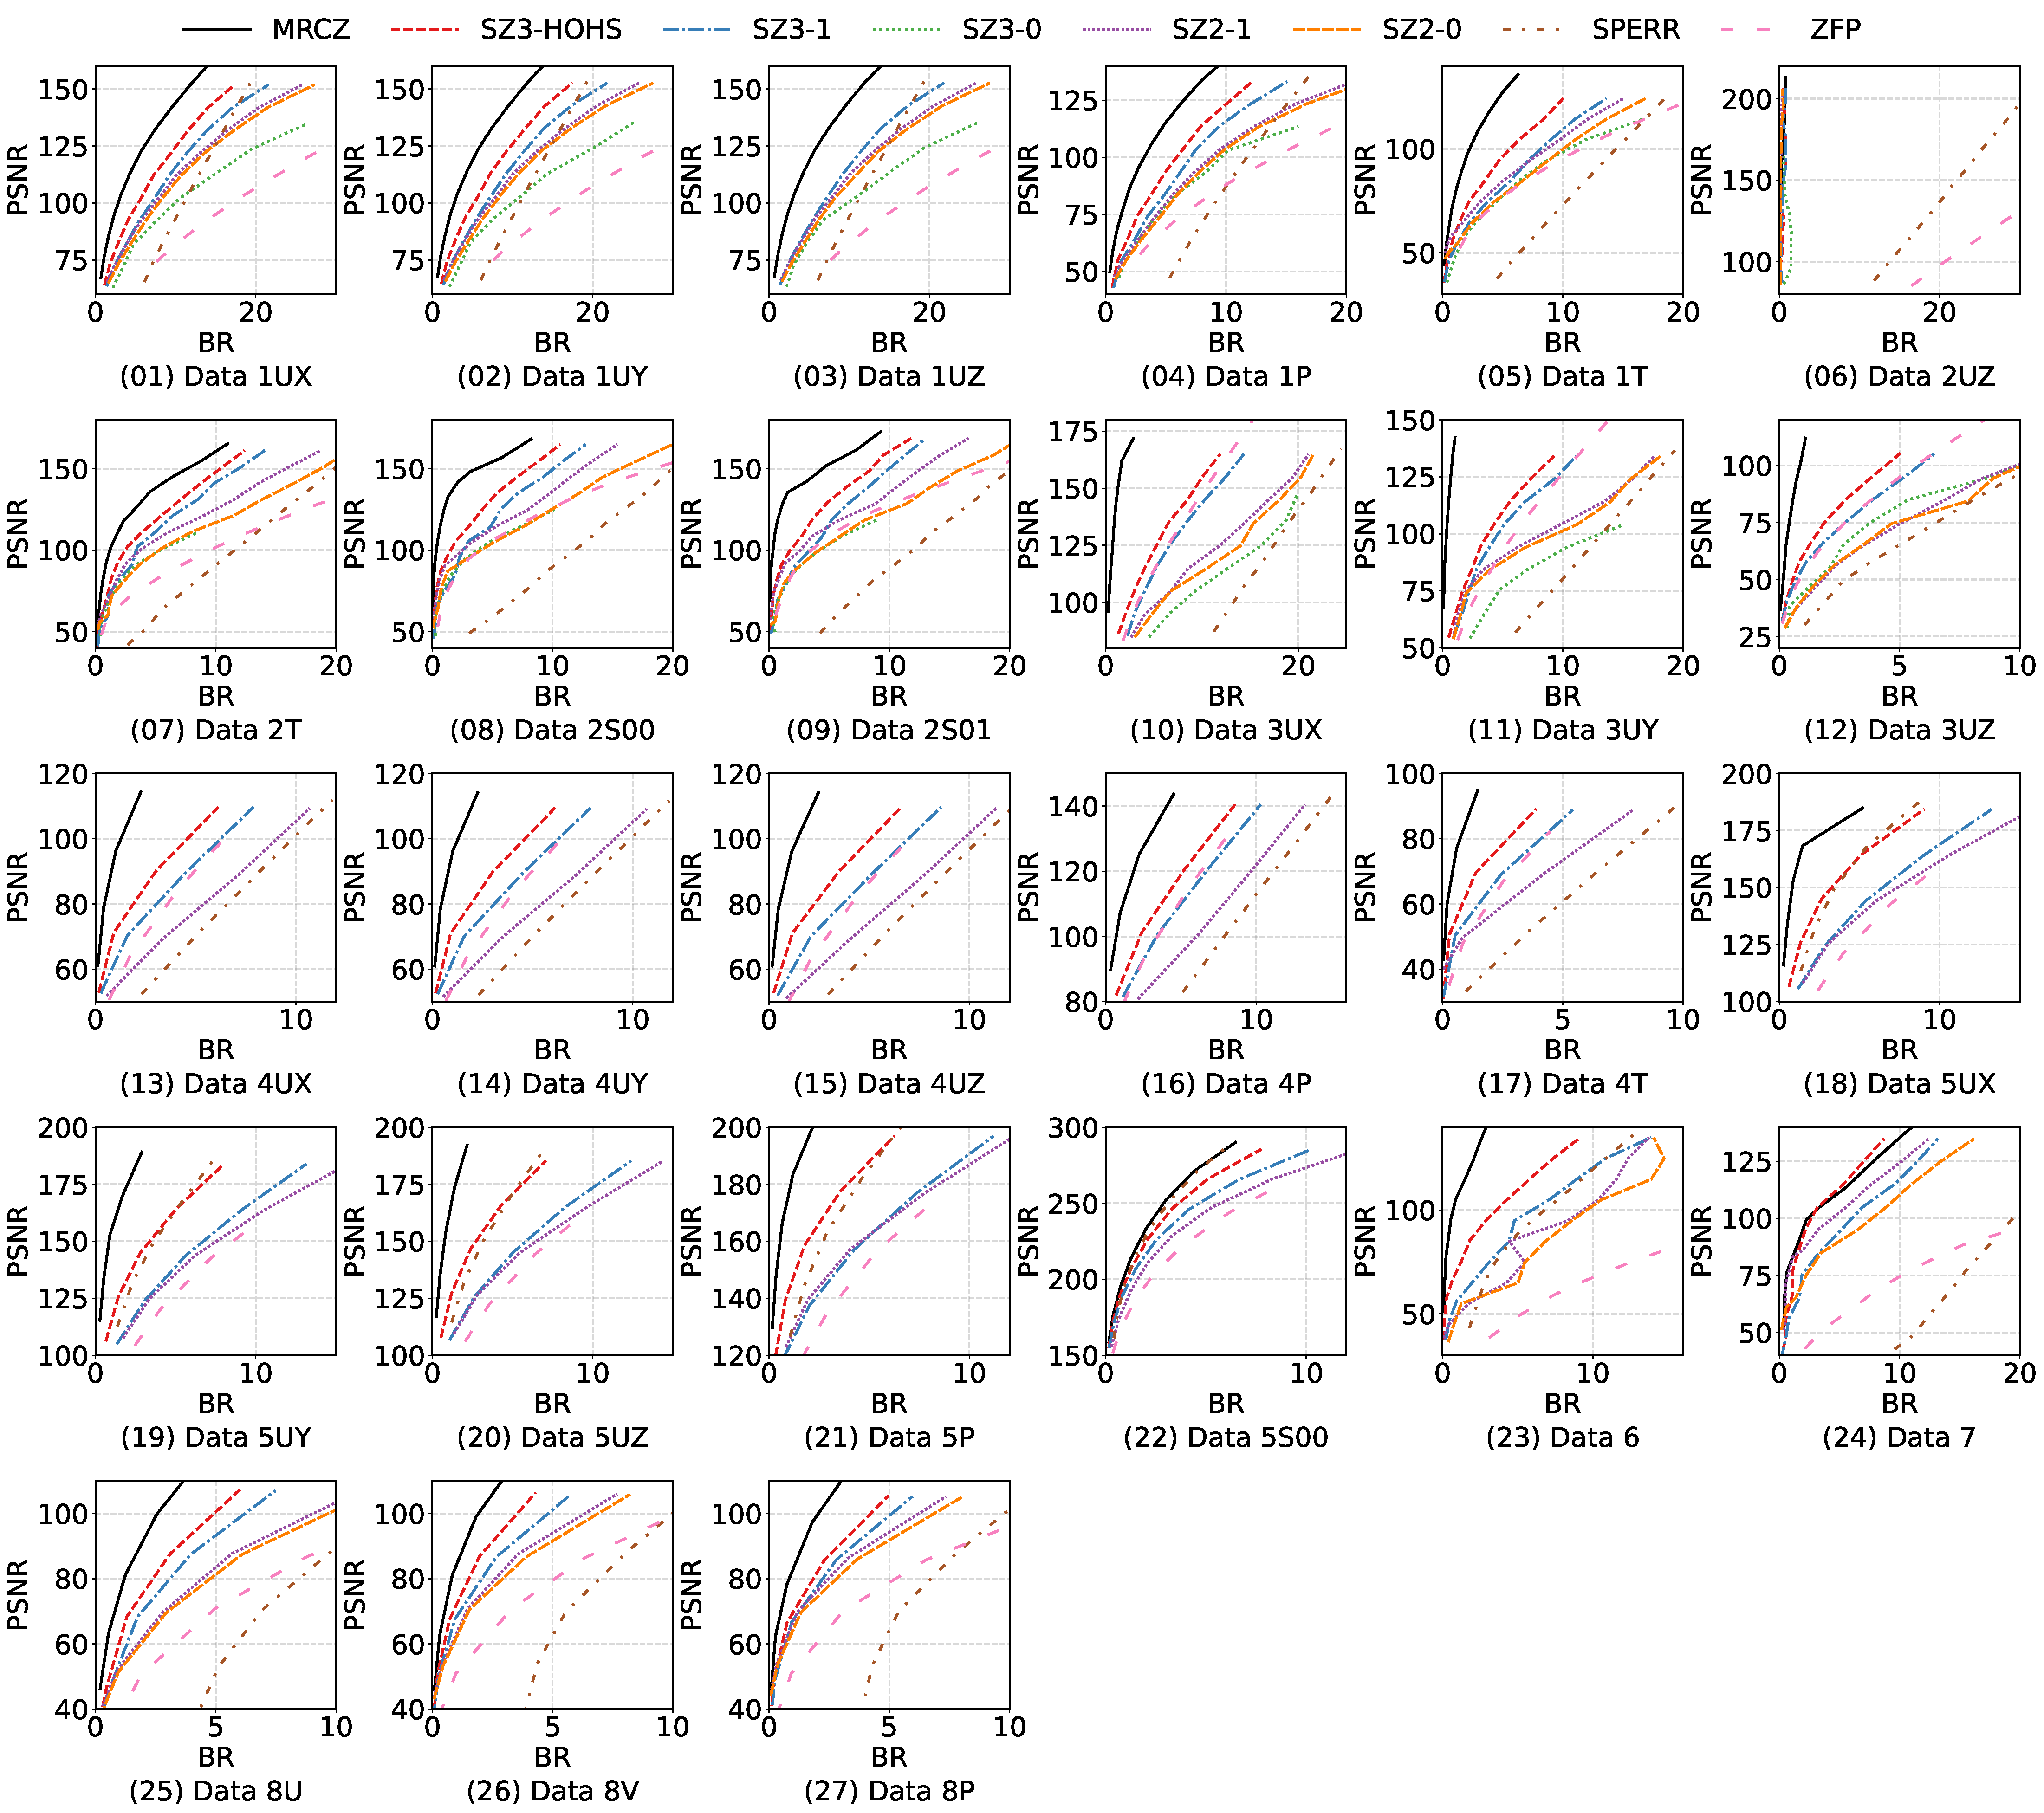
\includegraphics[width=1\textwidth]{figs/7/rd.pdf}
    \caption{Evaluation of PSNR rate distortion curves between SZ3-HOHS, MRCZ, and baseline compressors.}
    \label{fig:rate-distortion}
\end{figure*}

Figure~\ref{fig:rate-distortion} presents the rate-distortion curves for all fields in Table~\ref{tab:datasets} across all evaluated compressors. These curves are used to evaluate storage reduction under comparable data quality. The X-axis shows the bit rate, measured in bits per data point. A lower bit rate indicates a smaller compressed representation. The Y-axis shows PSNR as a numerical measure of reconstruction quality. Therefore, for a fixed PSNR, a curve farther to the left indicates better storage reduction. Equivalently, for a fixed bit rate, a curve higher on the plot indicates better reconstruction quality. Overall, better performance is indicated by curves closer to the upper-left.

Overall, \textbf{\textit{SZ3-HOHS and MRCZ consistently outperform all baseline lossy compressors}}. MRCZ achieves the best rate-distortion performance for 26 out of 27 HOHS fields, while SZ3-HOHS achieves the second-best curve for 23 out of 27 fields. These results demonstrate that, compared with the baseline compressors, the proposed methods consistently provide greater storage reduction while maintaining comparable reconstruction quality across diverse HOHS datasets.

The performance improvements originate from different design mechanisms in the two proposed methods.
SZ3-HOHS achieves better performance by employing distance-aware interpolation weights based on the GLL point distribution in the reference element, leading to more accurate predictions.
MRCZ improves compressibility by using a more effective transform that produces more concentrated coefficients. This allows MRCZ to use a smaller coefficient error bound without introducing excessive coefficient-storage overhead. Meanwhile, a smaller coefficient error bound improves the inverse-transform reconstruction accuracy, producing smaller and more concentrated residuals that are easier to compress. Finally, MRCZ reorganizes the quantized coefficients across elements to improve their continuity before lossless encoding, further reducing the final bit rate.

% Some baseline compressors also produce less stable rate-distortion curves. For example, on dataset 6, SZ2-0 and SZ2-1 occasionally increase bit rate while reducing PSNR. In contrast, SZ3-HOHS and MRCZ produce smoother and more predictable rate-distortion curves across diverse HOHS fields.

To further quantify storage reduction under practical error-bound settings, we report compression ratios for two representative fields, 4UX (3.71 GB) and 5P (12.07 GB), in Table~\ref{tab:compression-ratios}. Unlike the rate-distortion curves in Figure~\ref{fig:rate-distortion}, which compare methods under PSNR-based reconstruction quality, this table evaluates compression ratios under fixed pointwise error bounds. Due to the different value ranges of the two fields, they are evaluated under different absolute error bounds. We report SZ3-1 and SZ2-1 as the adapted SZ baselines, while omitting SZ3-0 and SZ2-0 due to their poor rate-distortion performance.

\begin{table*}[h]
    \centering
    \caption{Compression ratios of two leading fields 4UX and 5P across all evaluated lossy compressors. The SZ3-0 and SZ2-0 are excluded due to sacrificed performance. The \textbf{highest} and \underline{second-highest} compression ratios are highlighted.}
    \label{tab:compression-ratios}
    \begin{tabular}{c|c|cccccccc}\toprule
        \textbf{HOHS Field} & \textbf{Error Bound} & \textbf{MRCZ}    & \textbf{SZ3-HOHS} & \textbf{SZ3-1}   & \textbf{SZ2-1}  & \textbf{SPERR}  & \textbf{ZFP} \\
        \midrule
        4UX                     & ABS 1E-1   & \textbf{255.387} & \underline{191.789}  & 118.431 & 57.841 & 13.891 & 7.697\\
        4UX                     & ABS 1E-2   & \textbf{79.910}  & \underline{34.870}   & 20.134  & 9.435  & 6.098  & 4.855\\
        4UX                     & ABS 1E-3   & \textbf{31.391}  & \underline{10.625}   & 7.092   & 4.440  & 3.770  & 3.414\\
        \midrule
        5P                      & ABS 1E-4   & \textbf{196.138} & \underline{97.935}   & 44.649  & 37.830 & 30.479 & 5.932\\
        5P                      & ABS 1E-5   & \textbf{92.083}  & \underline{39.329}   & 15.864  & 16.587 & 17.871 & 3.952\\
        5P                      & ABS 1E-6   & \textbf{48.883}  & \underline{18.094}   & 7.557   & 7.871  & 10.999 & 2.788\\\bottomrule
    \end{tabular}
\end{table*}

Table~\ref{tab:compression-ratios} shows the storage-reduction performance under fixed error-bound constraints. We can find that \textbf{\textit{MRCZ and SZ3-HOHS consistently achieve the highest compression ratios across all reported cases.}} MRCZ achieves up to 5.47$\times$ higher compression ratio than SZ3-1, the strongest baseline in this comparison, while SZ3-HOHS consistently delivers the second-best compression ratios. These results show that the proposed methods are effective not only under PSNR-based rate-distortion evaluation, but also under the pointwise error-bound settings.

\subsection{End-to-End Workflow Evaluation}

In this subsection, we assess the practical impact of compression on end-to-end data movement between Purdue Anvil and Argonne Bebop using Globus~\cite{chard2017globus}, a widely used service for high-performance data transfer. For each evaluation, we compress all non-constant fields from HOHS Data 4 and 5 (Table~\ref{tab:datasets}) under an absolute error bound of $10^{-6}$, transfer the compressed data, and decompress it at the destination. The measured end-to-end time captures the trade-off between reduced transfer volume and compression/decompression overhead. Each dataset is evaluated three times, and the average results are reported.


\begin{figure}[htb]
    \centering
    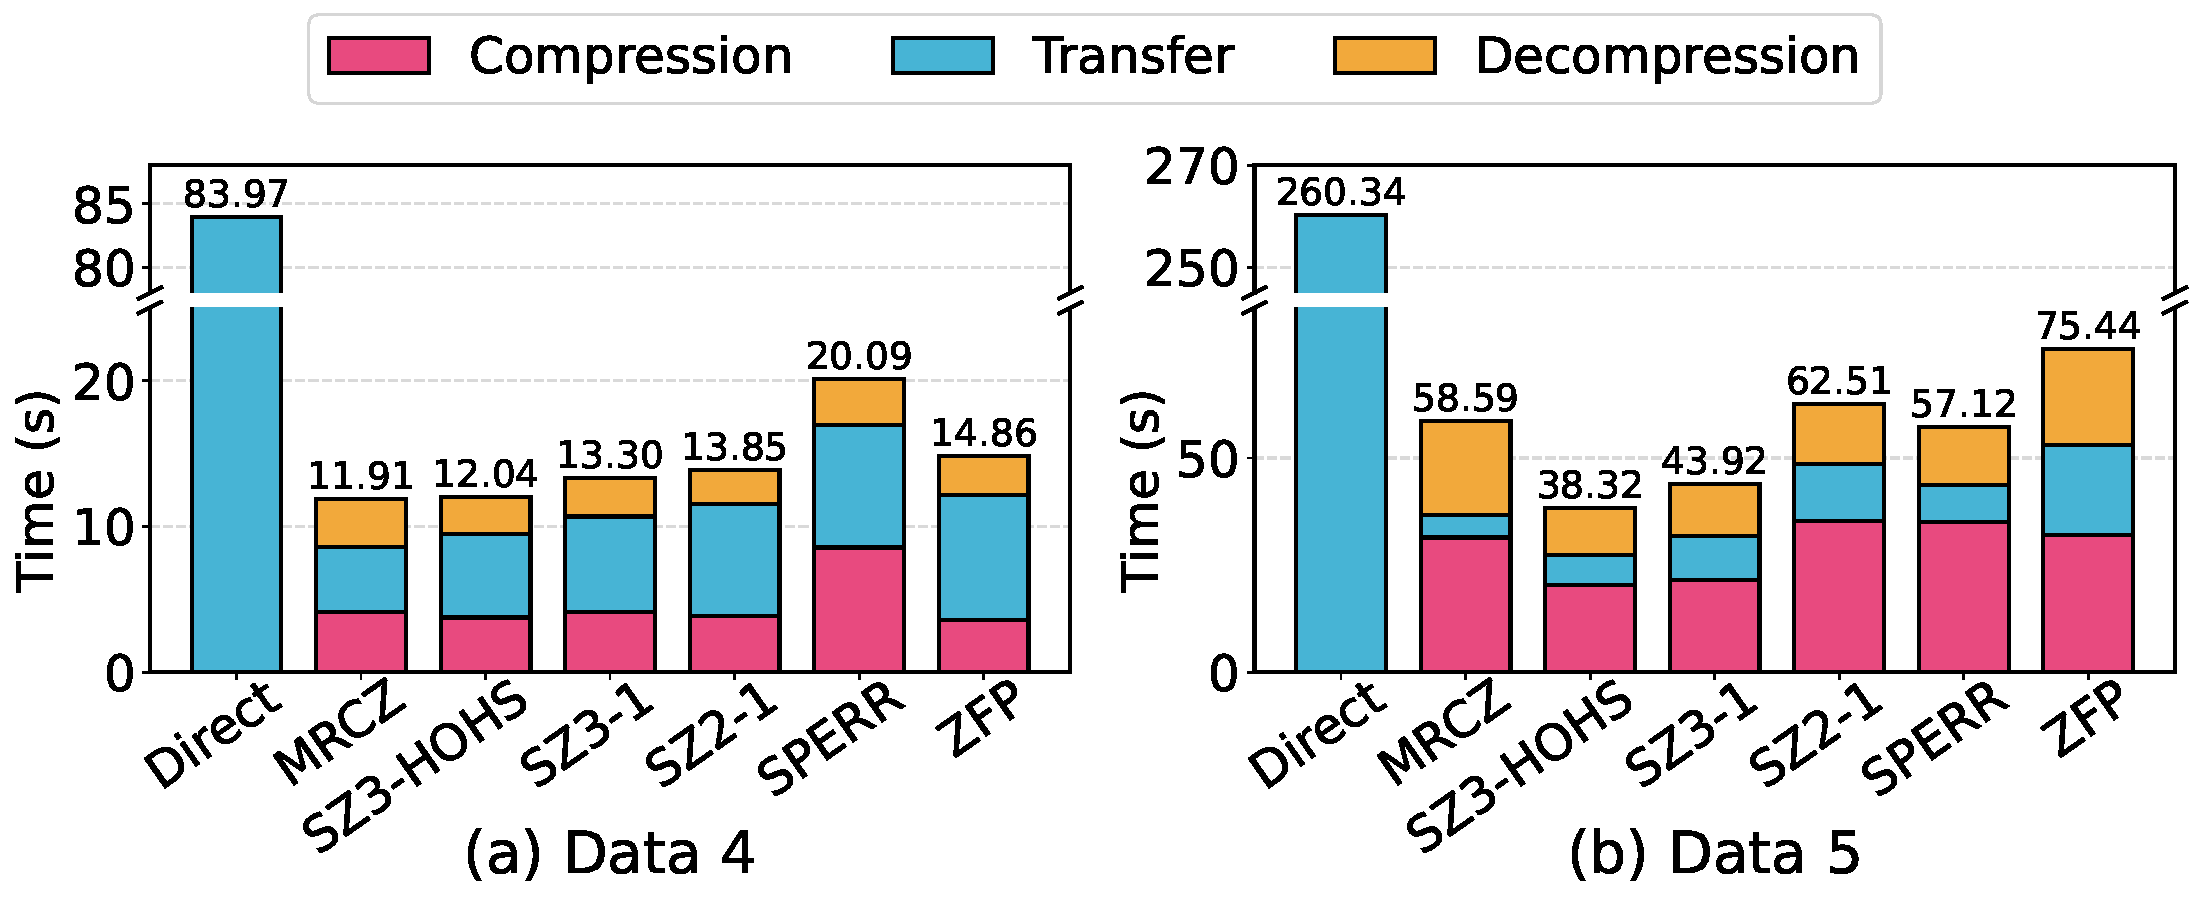
\includegraphics[width=1\linewidth]{figs/7/e2e_time.pdf}
    \caption{End-to-end Workflow Execution Time via Globus}
    \label{fig:transfer}
\end{figure}

As shown in Figure~\ref{fig:transfer}, MRCZ and SZ3-HOHS achieve the best end-to-end performance for Data 4 and Data 5, respectively, due to their high compression ratios and efficient implementations. For Data 4, MRCZ and SZ3-HOHS achieve end-to-end transfer times of 11.91 and 12.04 seconds, respectively. For Data 5, SZ3-HOHS is significantly faster than the other evaluated methods, requiring only 38.32 seconds, because it combines a high compression ratio with low computational overhead. \textit{\textbf{Overall, these results demonstrate the strong capability of SZ3-HOHS and MRCZ to reduce data-movement overhead for cross-facility scientific workloads.}}

\subsection{Parallel Throughput}\label{sec:parallel-throughput}

Following the end-to-end workflow evaluation, we further isolate the compression and decompression stages to examine their parallel scalability. Specifically, we conduct a strong-scaling evaluation of OpenMP compression and decompression throughput across all non-constant fields of Datasets 4 and 5 under an absolute error bound of $10^{-6}$. The number of threads is increased up to 128 while the input data size remains fixed. Each field is evaluated three times at each thread count, and we report the harmonic mean of all measured throughput values. Because all fields within each dataset have the same size, this is equivalent to dividing the aggregate processed data size by the aggregate execution time.

\begin{figure}[htb]
    \centering
    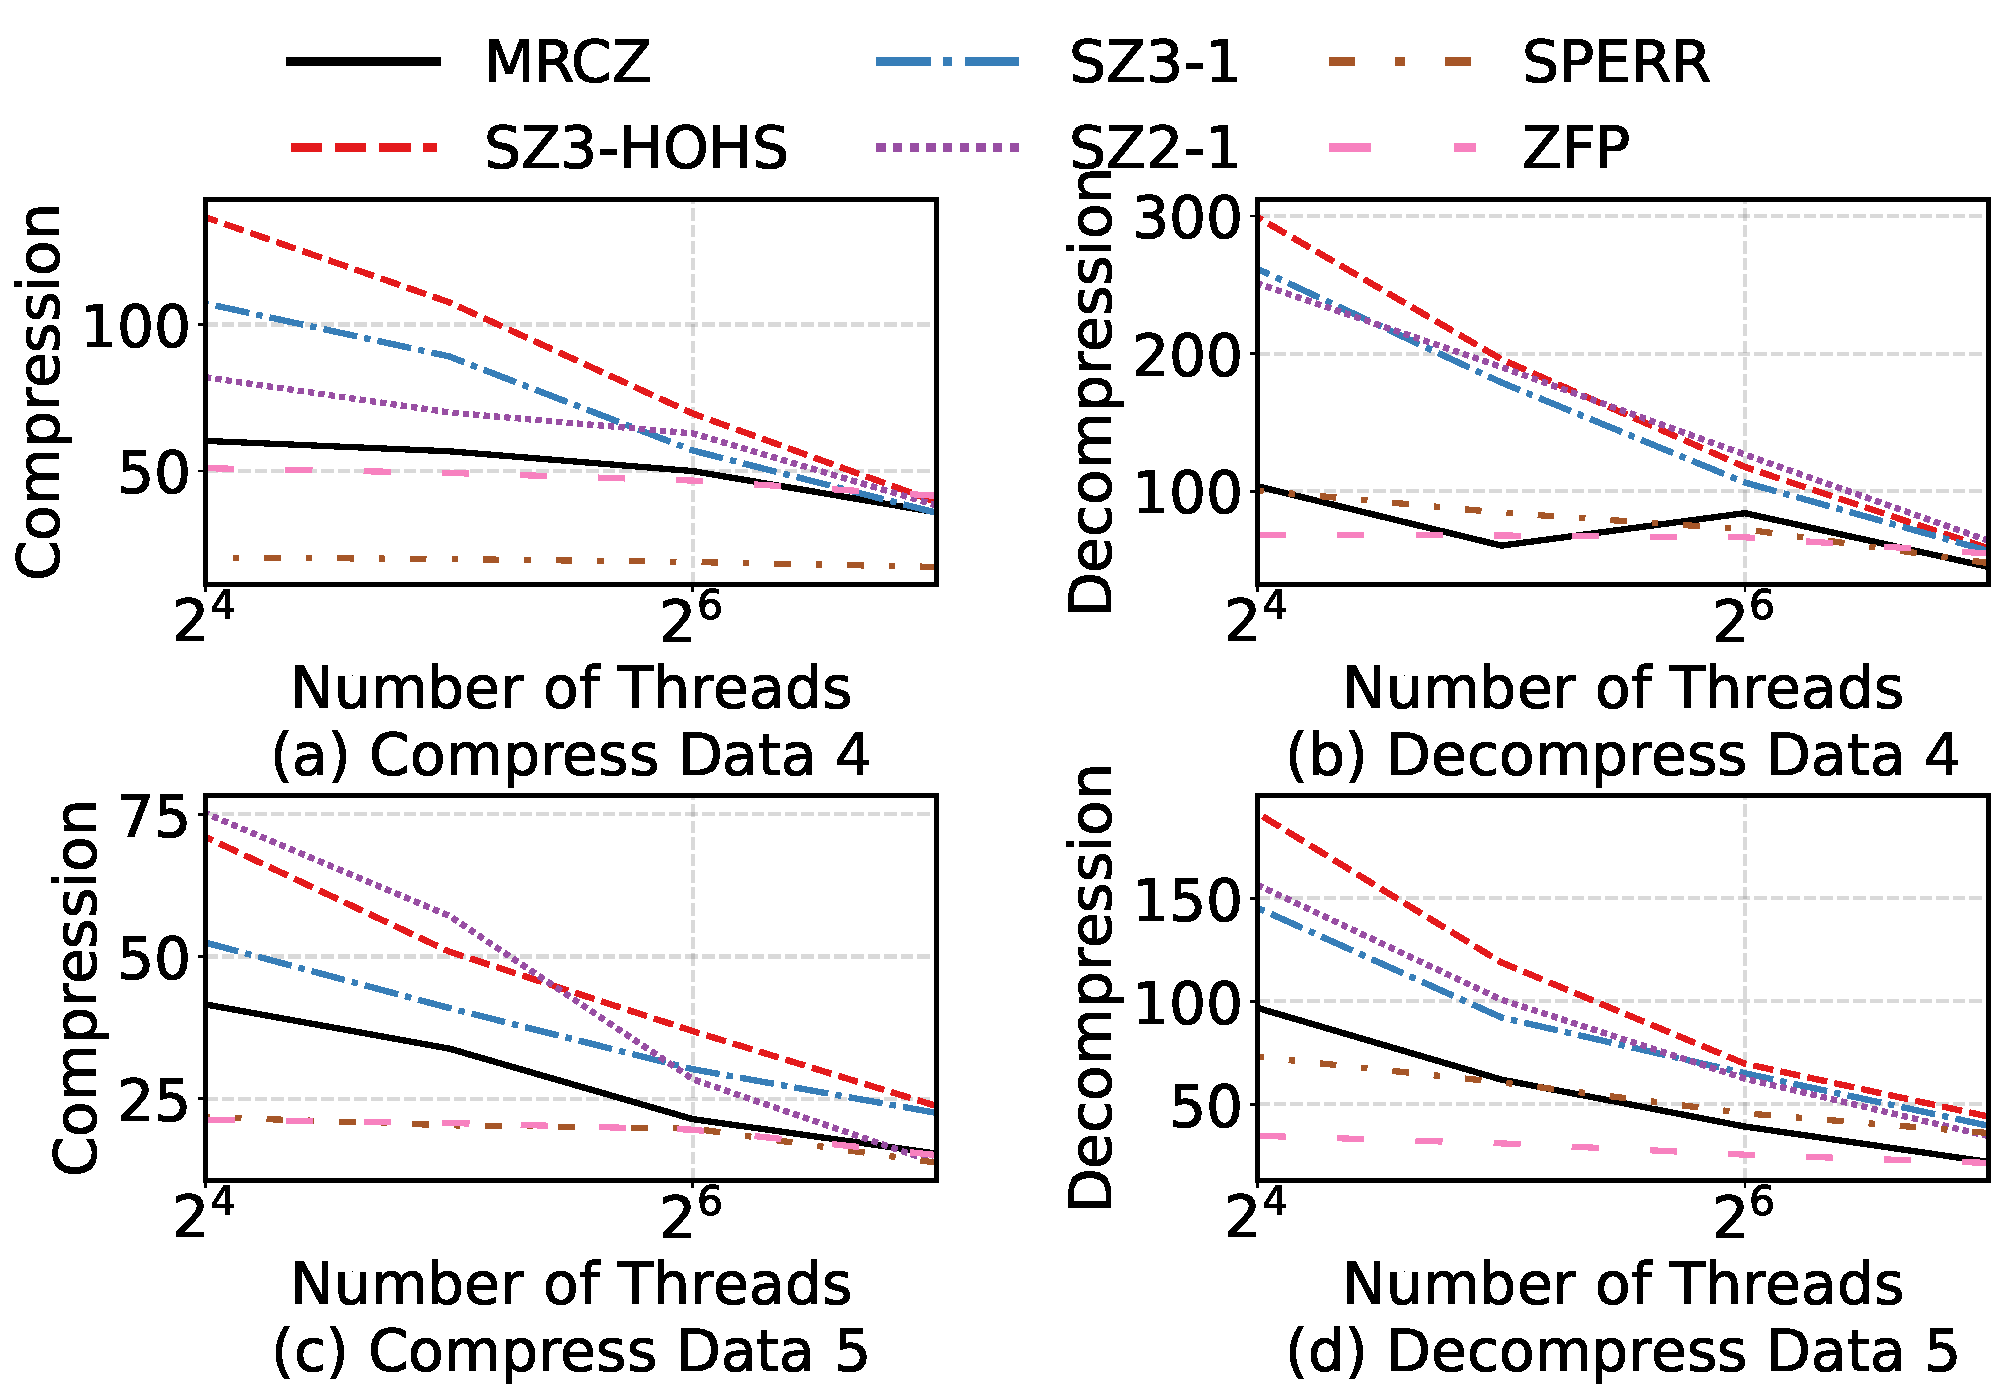
\includegraphics[width=0.9\linewidth]{figs/8-fig9.pdf}
    \caption{Parallel Execution Throughput (MB/s)}
    \label{fig:throughput}
\end{figure}

The results are shown in Figure~\ref{fig:throughput}. \textit{\textbf{SZ3-HOHS achieves the highest overall throughput, particularly during decompression, while MRCZ remains competitive despite its more computationally intensive transform-based prediction.}} For example, with 16 threads on Dataset 4, SZ3-HOHS and MRCZ achieve per-thread compression throughputs of 136.55 and 60.33 MB/s, respectively. By comparison, SZ3-1, SZ2-1, SPERR, and ZFP achieve 107.18, 82.01, 20.57, and 51.01 MB/s, respectively. MRCZ therefore provides substantially higher throughput than SPERR and moderately higher throughput than ZFP, while also delivering a higher compression ratio. One contributing factor is its accurate prediction, which produces more concentrated quantization symbols and reduces the cost of the subsequent lossless encoding stage.

These results reveal a practical trade-off between compression effectiveness and computational performance. MRCZ is preferable when maximizing compression ratio is the primary objective, whereas SZ3-HOHS offers a stronger balance between compression ratio and throughput when execution time is more important.

As the thread count increases, the per-thread throughput of MRCZ, SPERR, and ZFP remains relatively stable because their higher arithmetic intensity makes them less sensitive to shared memory bandwidth. In contrast, the lightweight prediction in SZ3-HOHS becomes memory-bandwidth-bound at relatively small thread counts, causing its per-thread throughput to decrease even as aggregate throughput continues to improve.

\subsection{Visualization}\label{sec:performance evaluation:visualization}

In this part, we examine a slice of the temperature field from the fourth dataset (4T in Table~\ref{tab:datasets}). To assess reconstruction quality across different error-bounded lossy compressors, we plot the pointwise absolute reconstruction errors produced by each method. Lighter colors indicate smaller errors and therefore higher reconstruction fidelity. For a fair comparison, all compressors are evaluated at comparable compression ratios close to 26.07. Only a small spatial region is shown for clarity.

\begin{table}[htb]
    \centering
    \caption{Error bounds at a compression ratio of $\sim$26.07.}
    \label{tab:error-bound-visualization}
    \begin{tabular}{c|ccc}
        \toprule
        \textbf{Compressor} & \textbf{MRCZ} & \textbf{SZ3-HOHS} & \textbf{SZ3-1} \\
        \textbf{Relative Error Bound} & $1.04\times10^{-4}$ & $7.9\times10^{-4}$ & $2\times10^{-3}$ \\
        \midrule
        \textbf{Compressor} & \textbf{SZ2-1} & \textbf{ZFP} & \textbf{SPERR} \\
        \textbf{Relative Error Bound} & $4.2\times10^{-3}$ & $3.16\times10^{-1}$ & $4.52\times10^{-2}$ \\\bottomrule
    \end{tabular}
\end{table}

\begin{figure}[htb]
  \centering
  \begin{subfigure}[t]{0.45\linewidth}
    \centering
    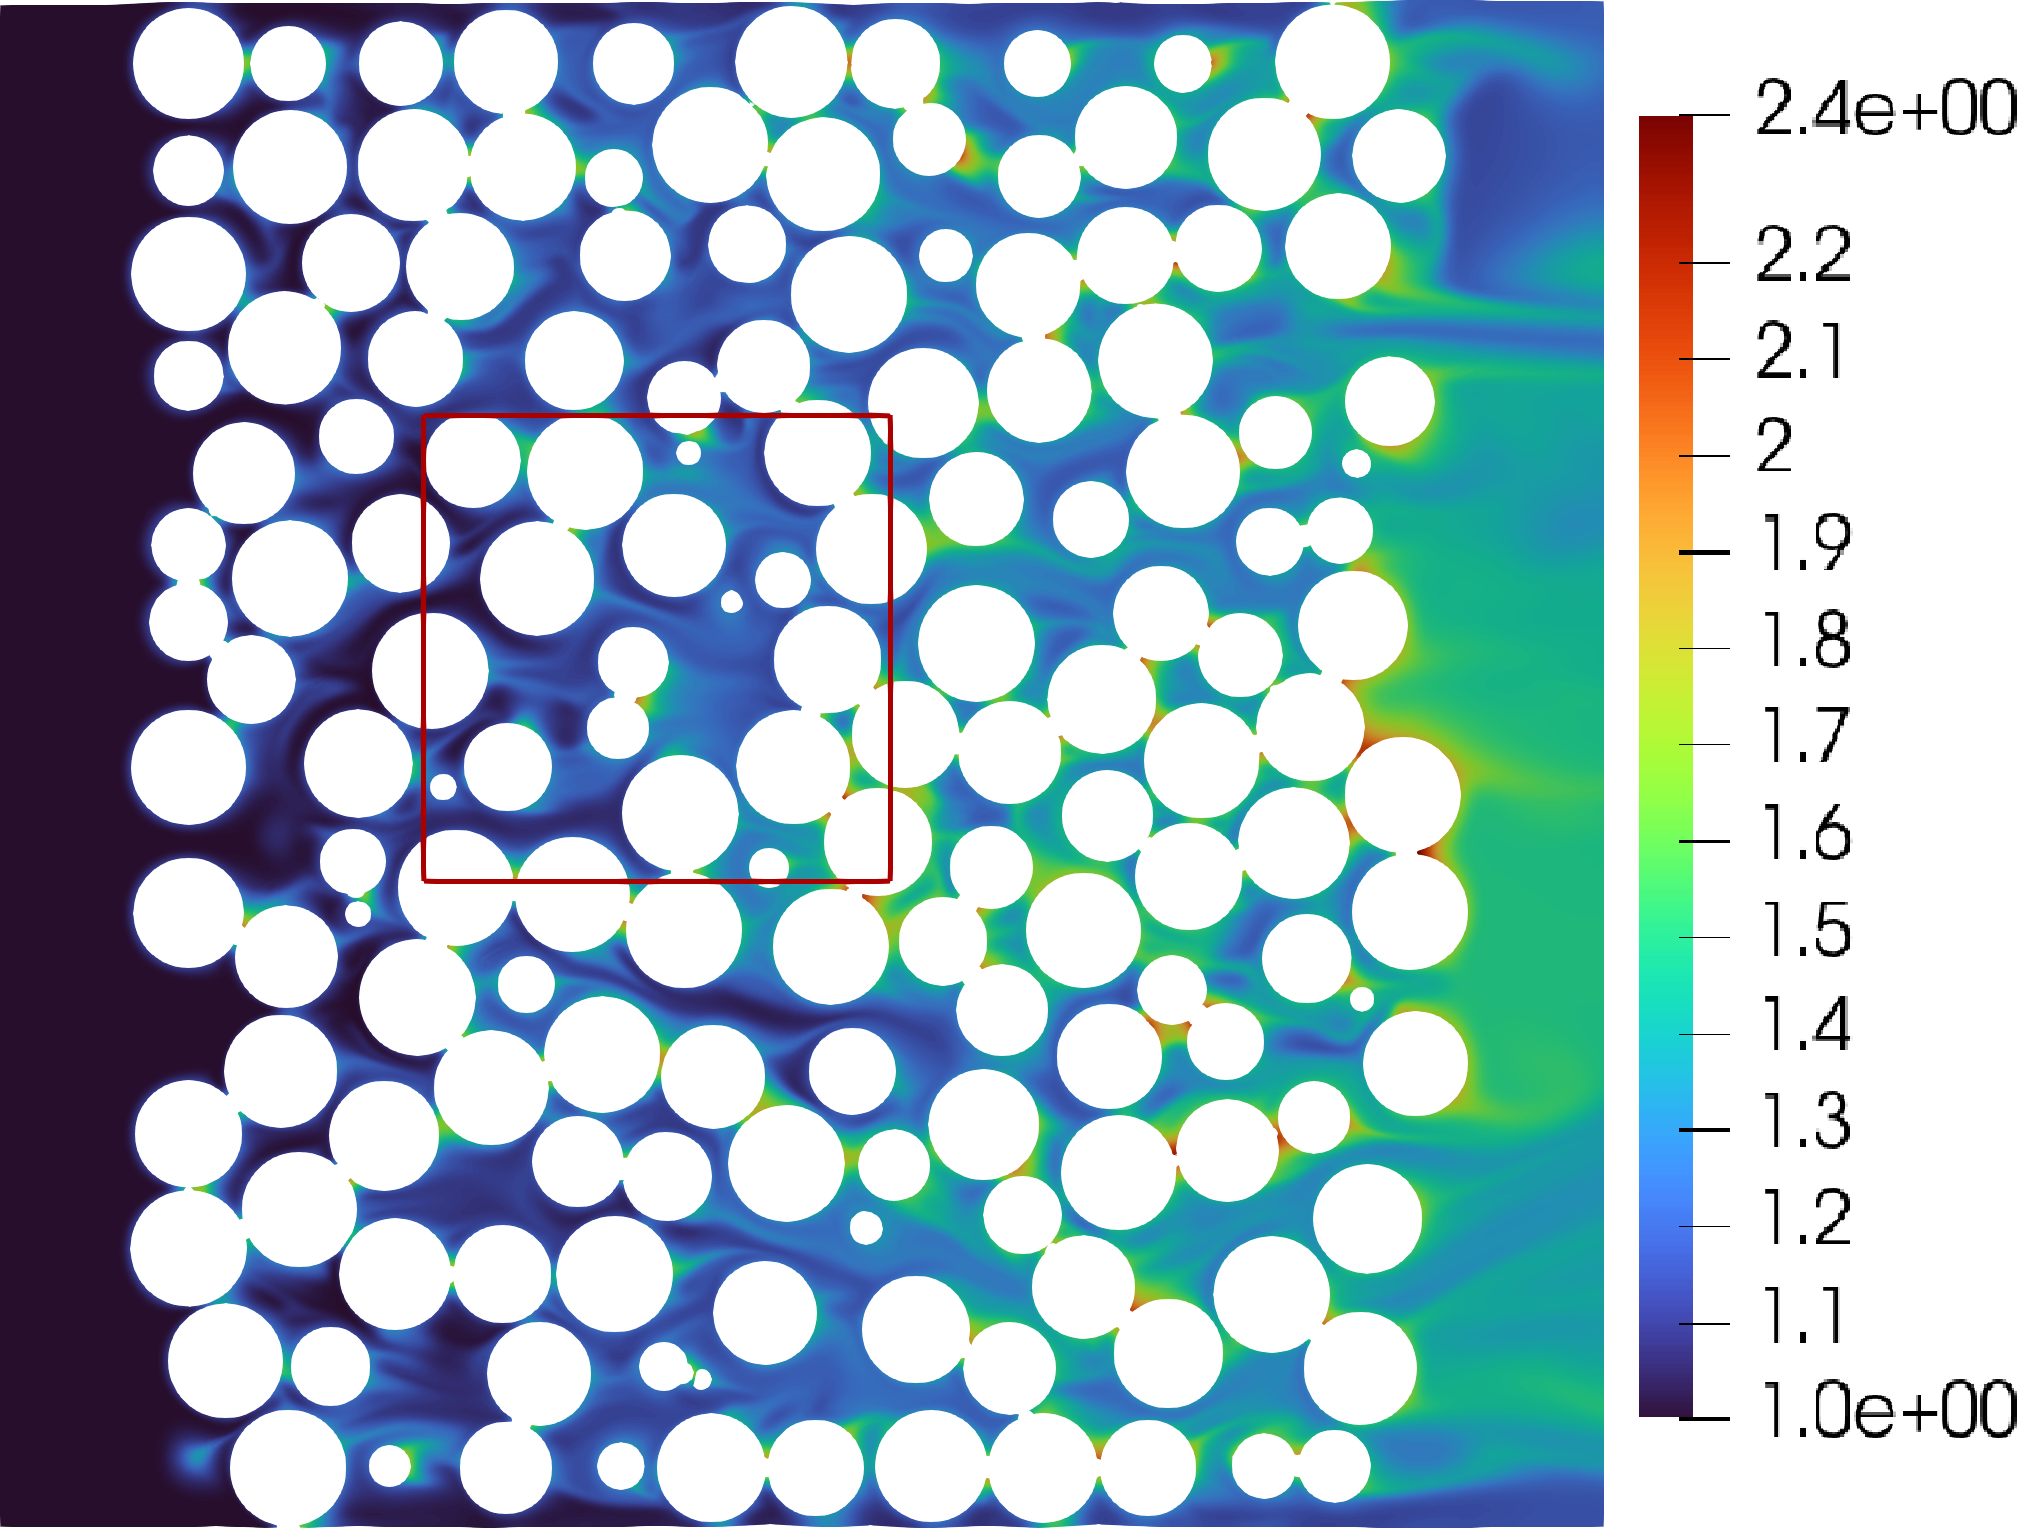
\includegraphics[width=\linewidth]{figs/7/pb0.png}
    \caption{Slice Visualization from 4T}
  \end{subfigure}
  \\
  \begin{subfigure}[t]{0.30\linewidth}
    \centering
    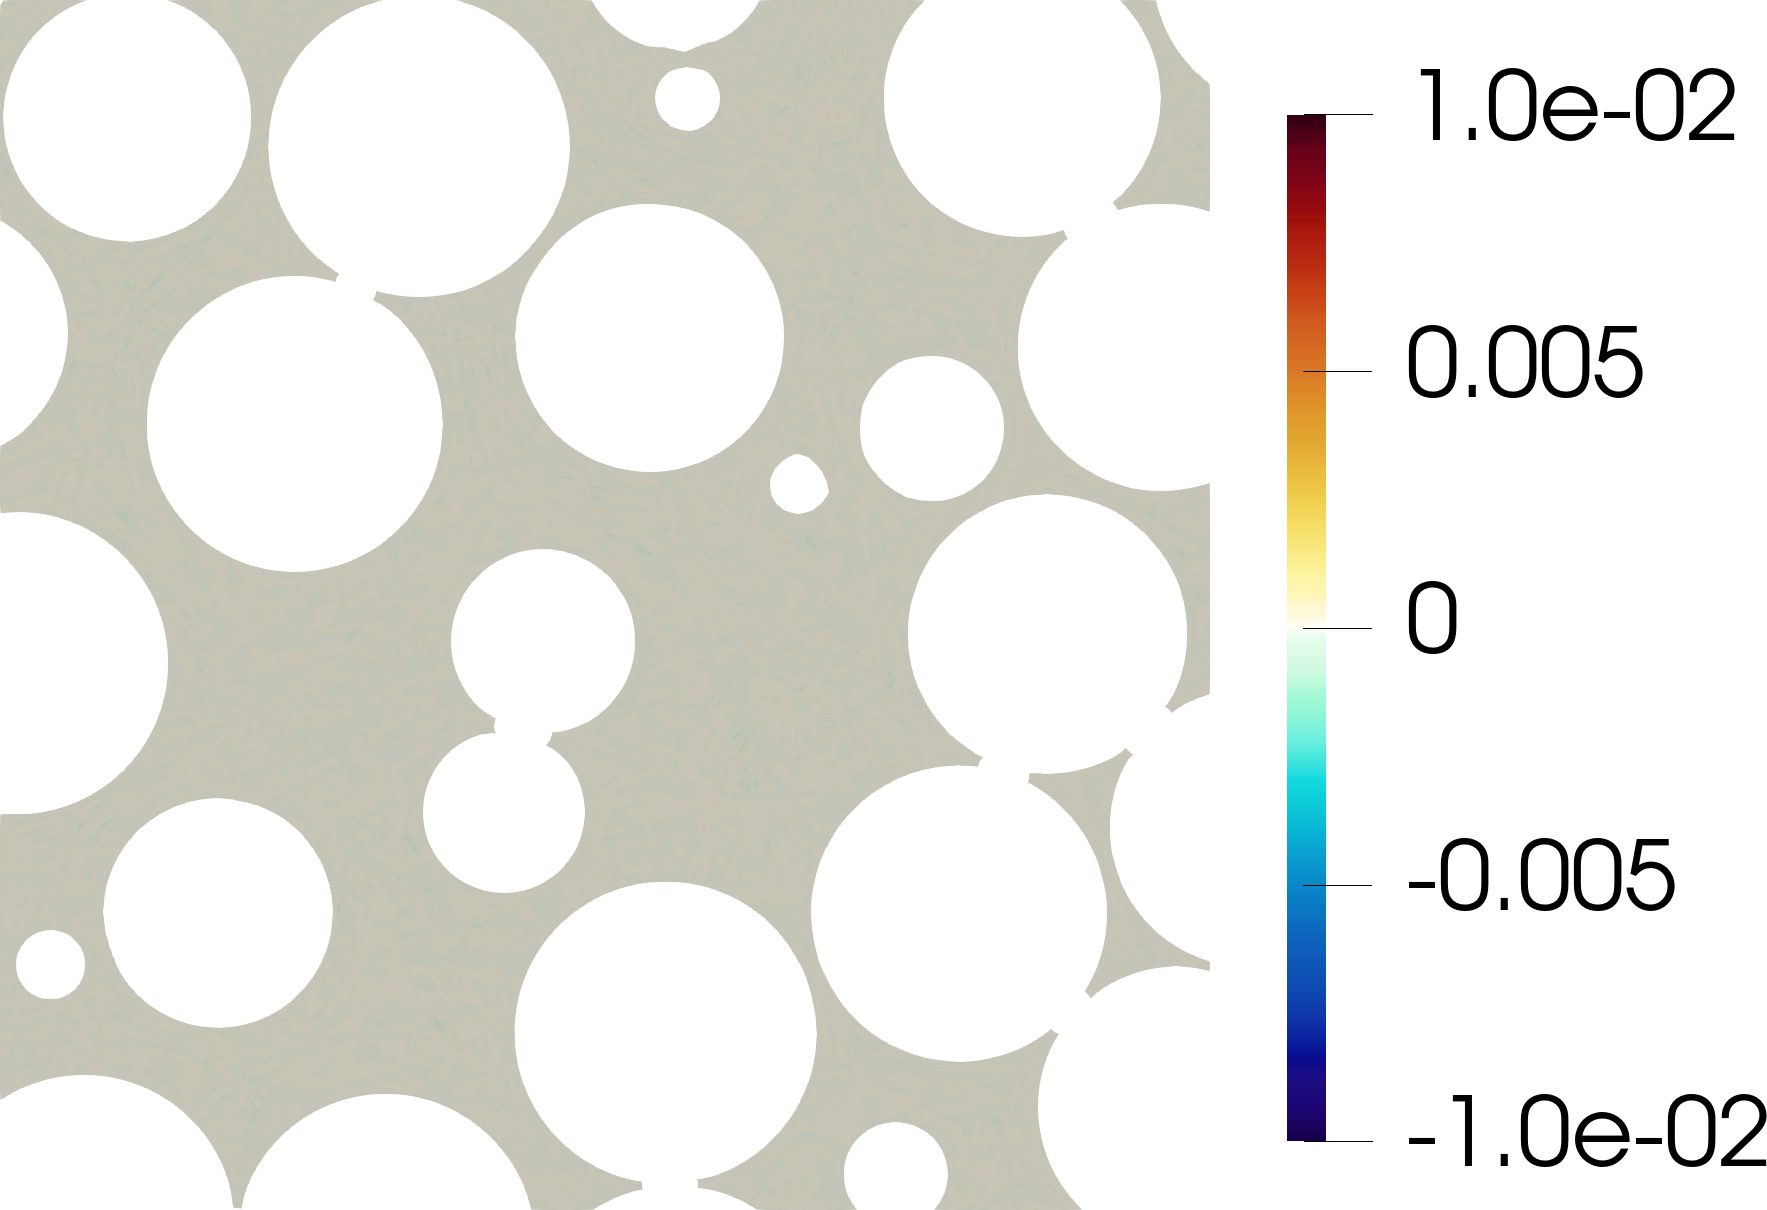
\includegraphics[width=\linewidth]{figs/7/mrcz err.png}
    \caption{MRCZ}
  \end{subfigure}
  \hfill
  \begin{subfigure}[t]{0.30\linewidth}
    \centering
    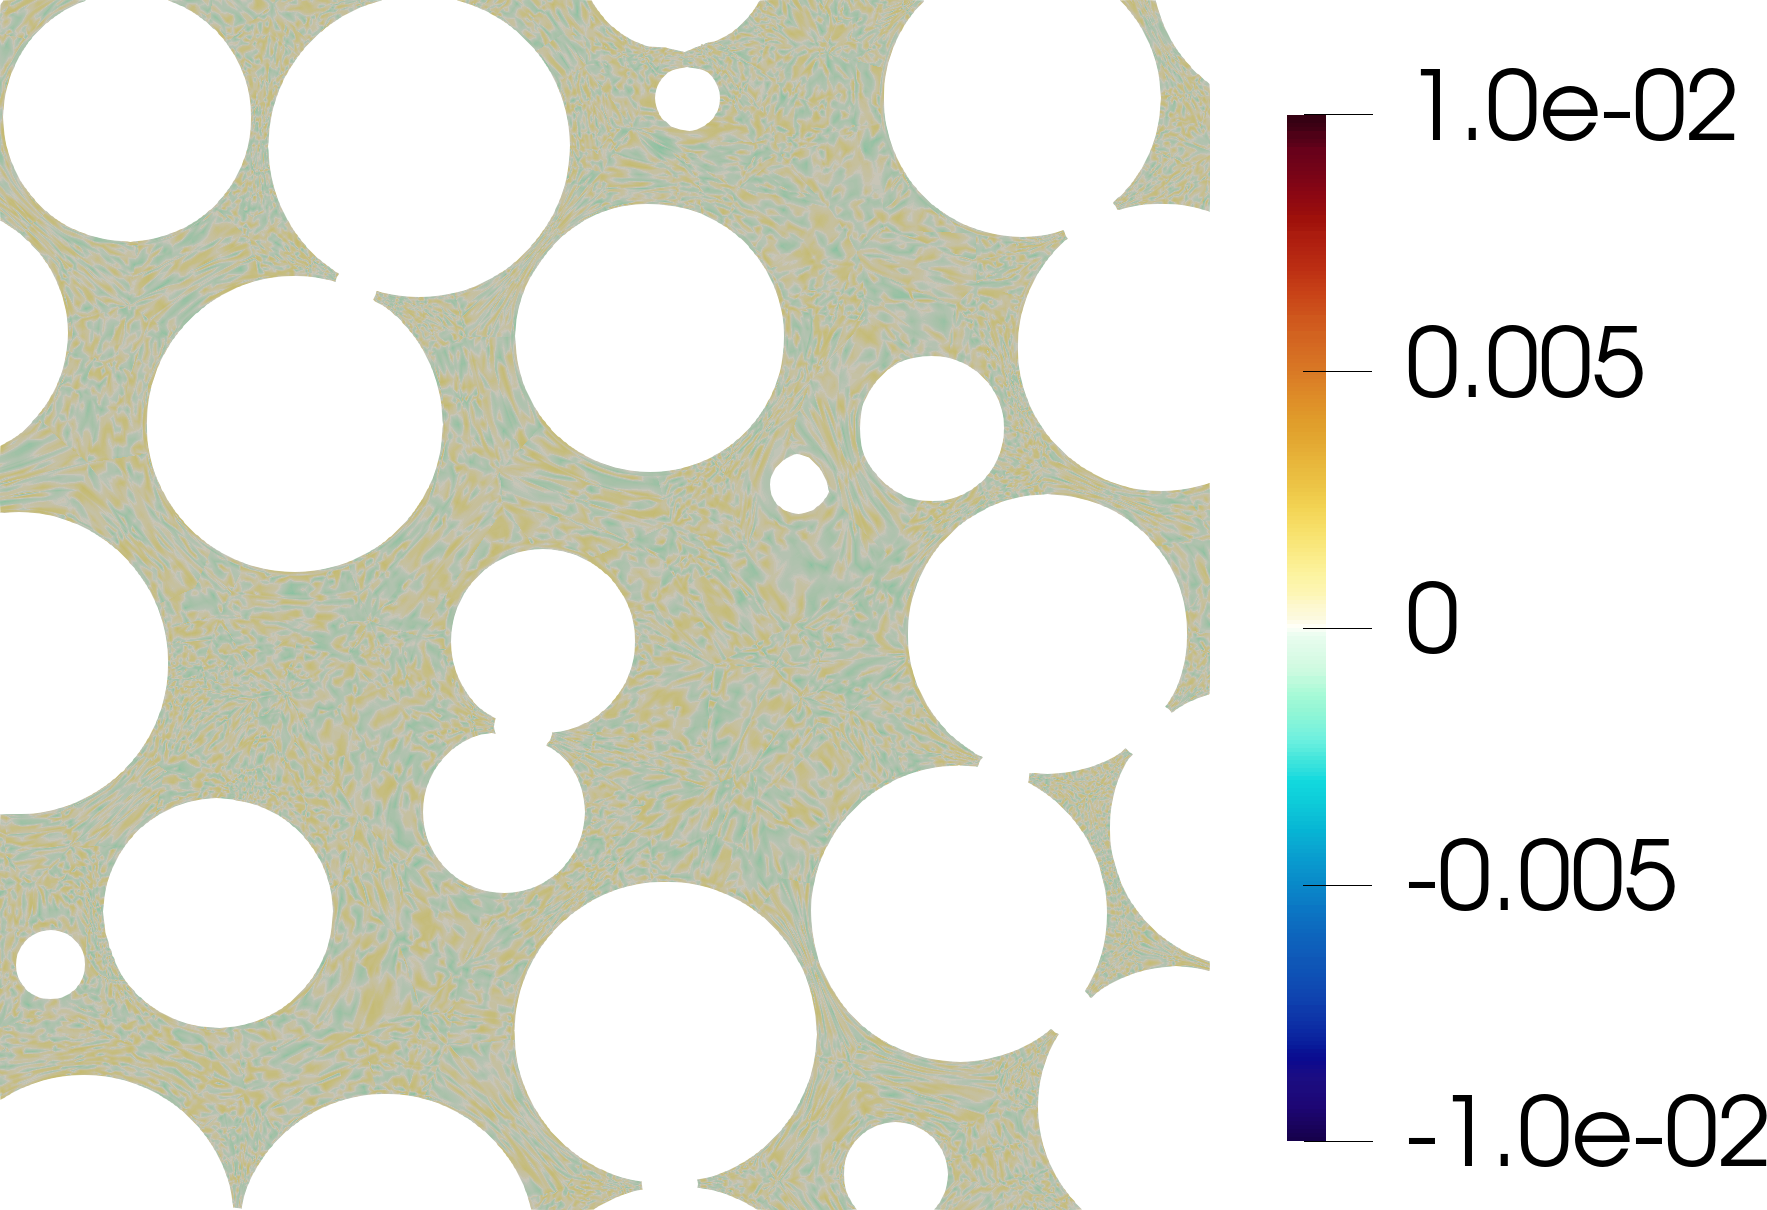
\includegraphics[width=\linewidth]{figs/7/sz3nekrs err.png}
    \caption{SZ3-HOHS}
  \end{subfigure}
  \hfill
  \begin{subfigure}[t]{0.30\linewidth}
    \centering
    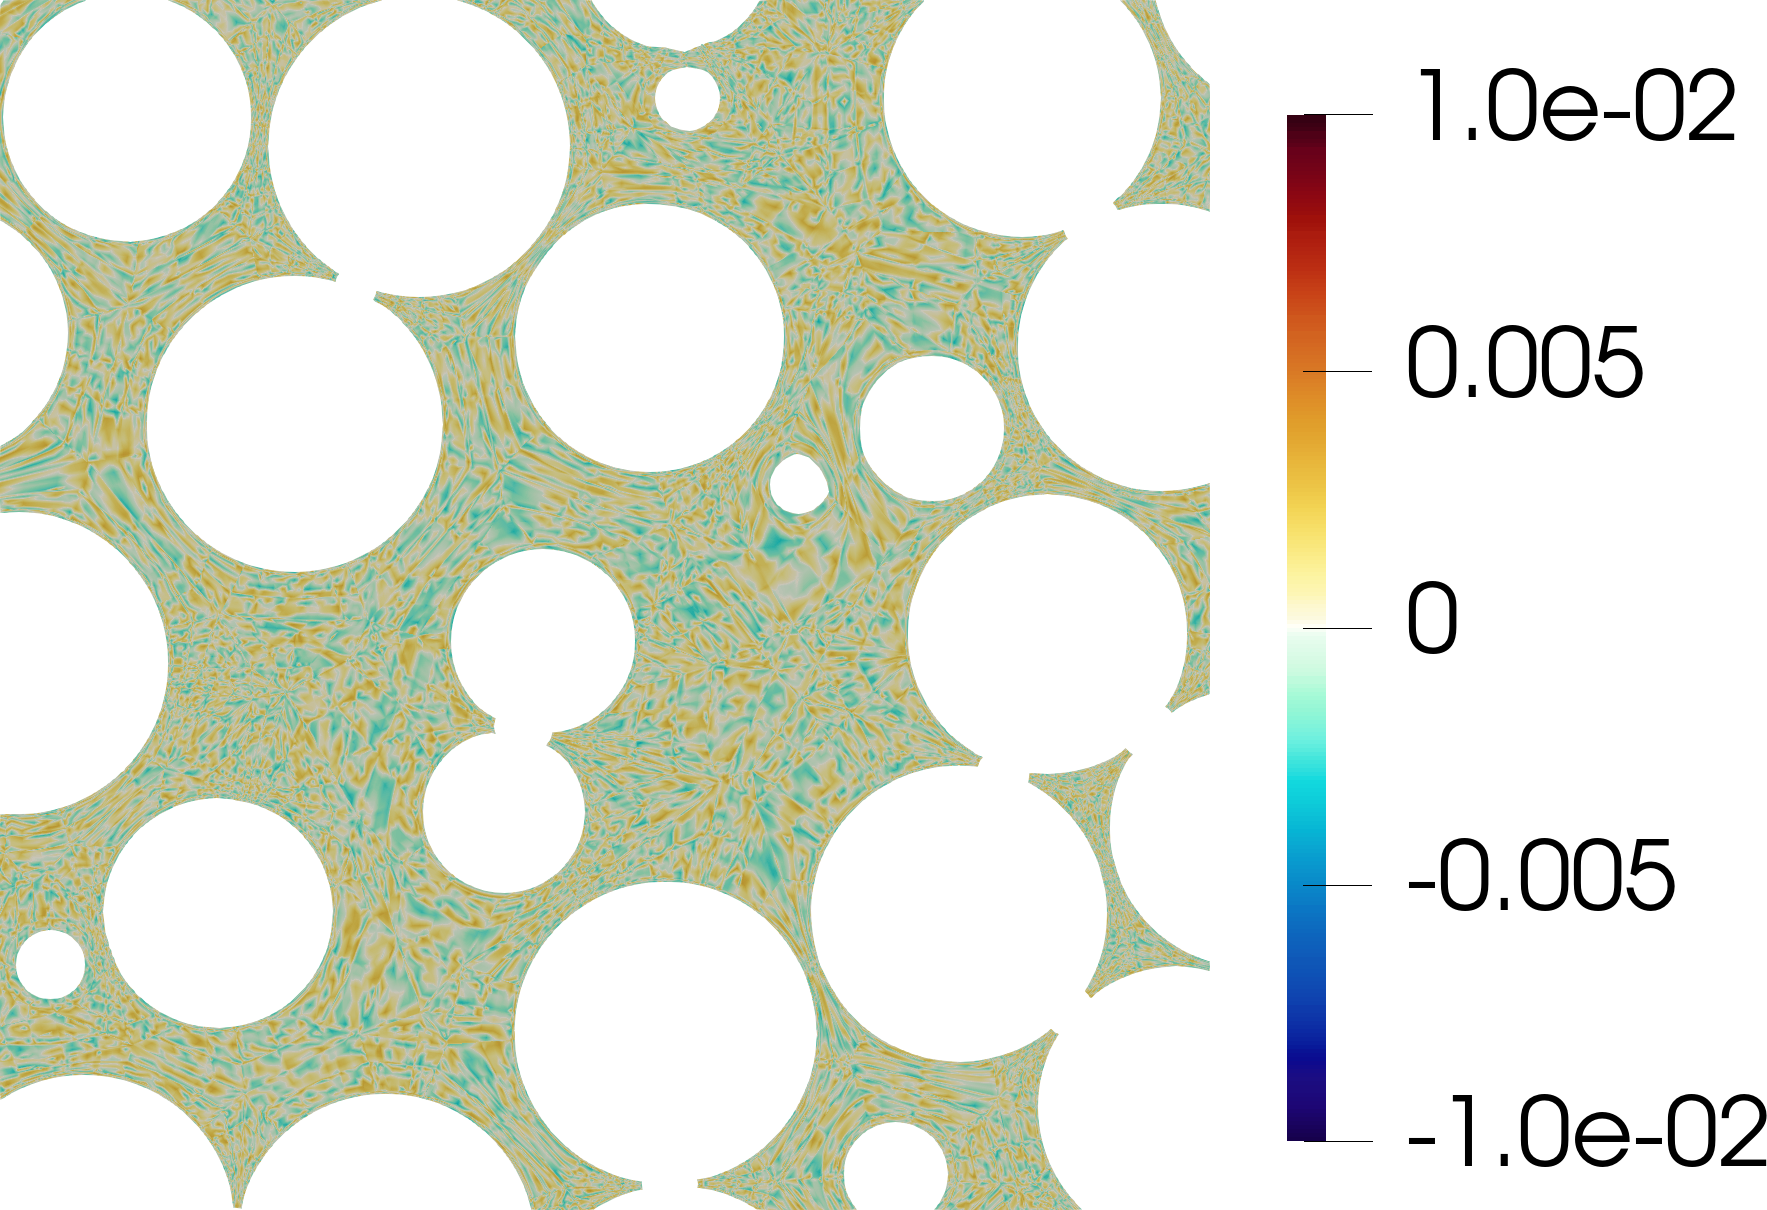
\includegraphics[width=\linewidth]{figs/7/sz3 err.png}
    \caption{SZ3-1}
  \end{subfigure}
  \\
  \begin{subfigure}[t]{0.30\linewidth}
    \centering
    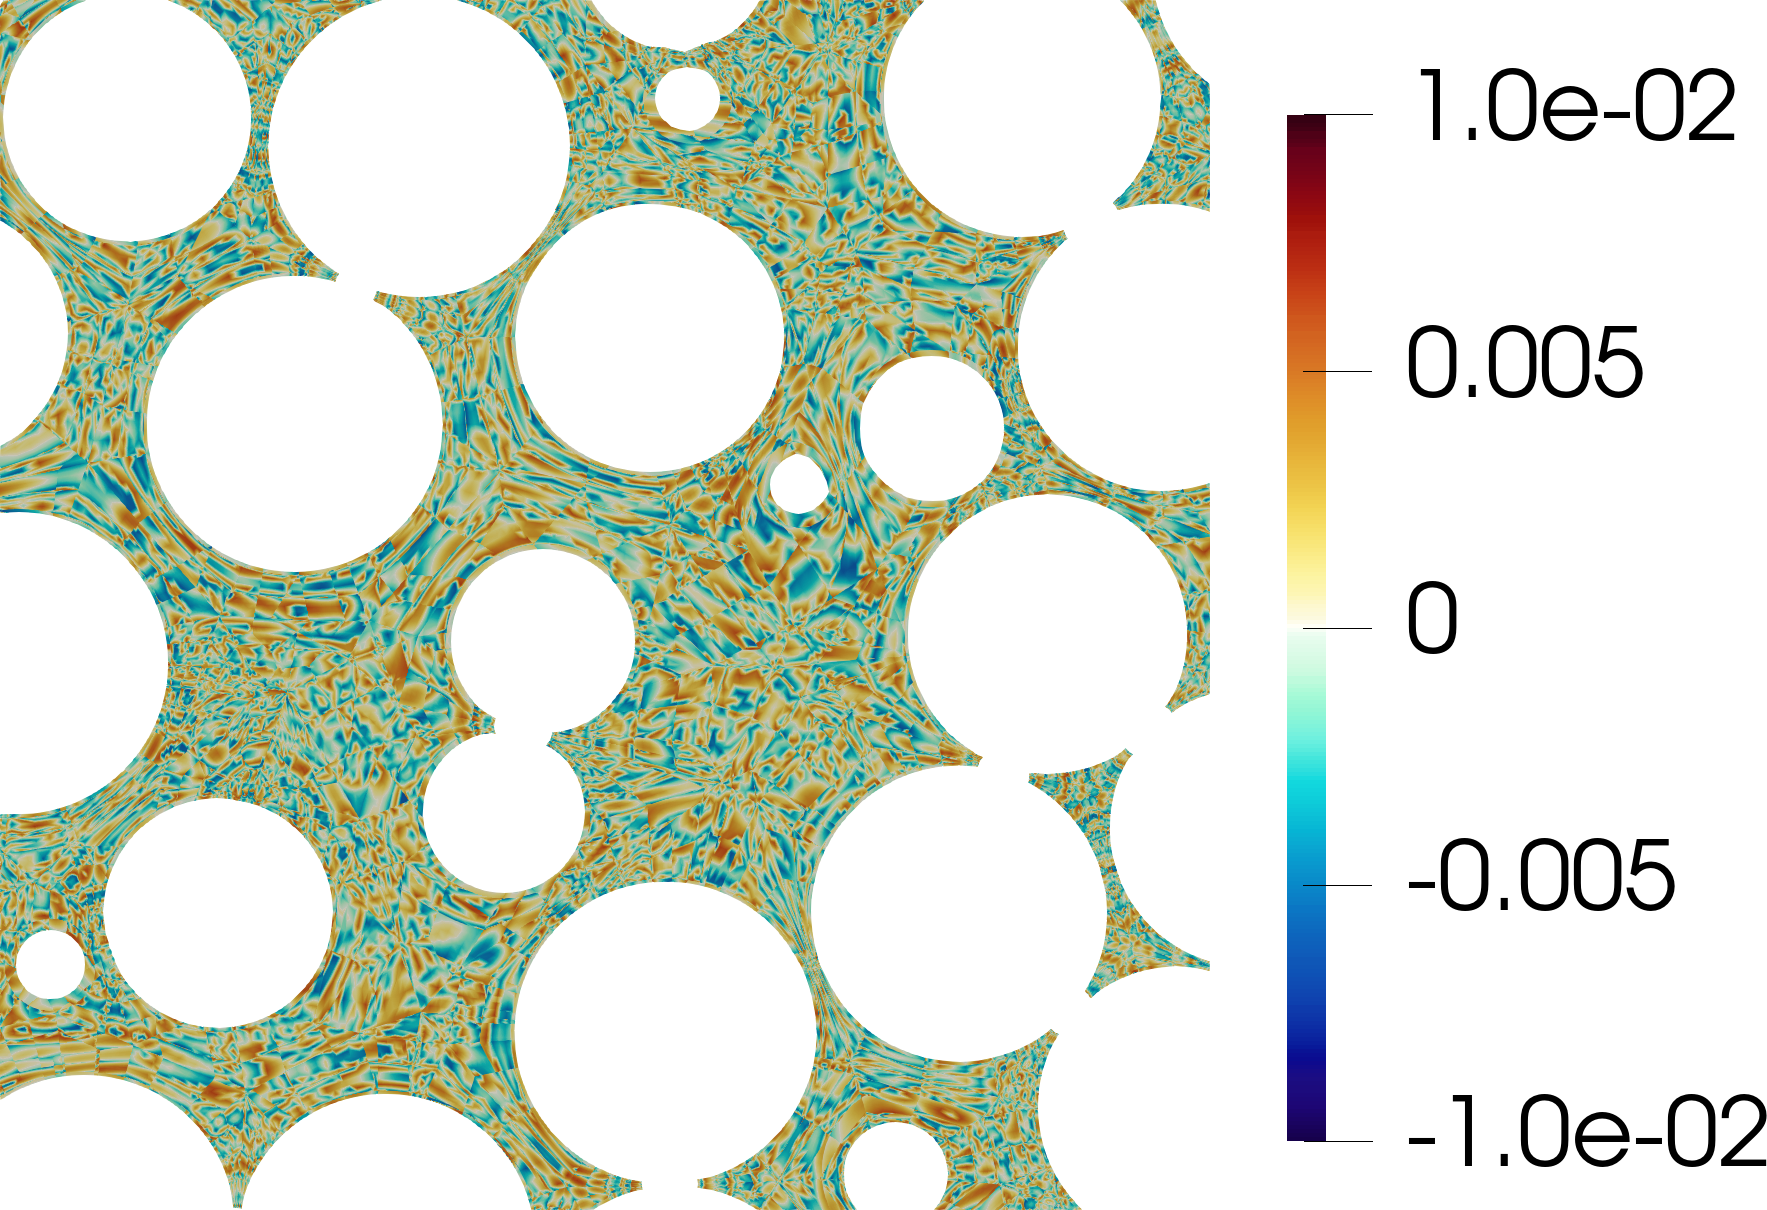
\includegraphics[width=\linewidth]{figs/7/sz2 err.png}
    \caption{SZ2-1}
  \end{subfigure}
  \hfill
  \begin{subfigure}[t]{0.30\linewidth}
    \centering
    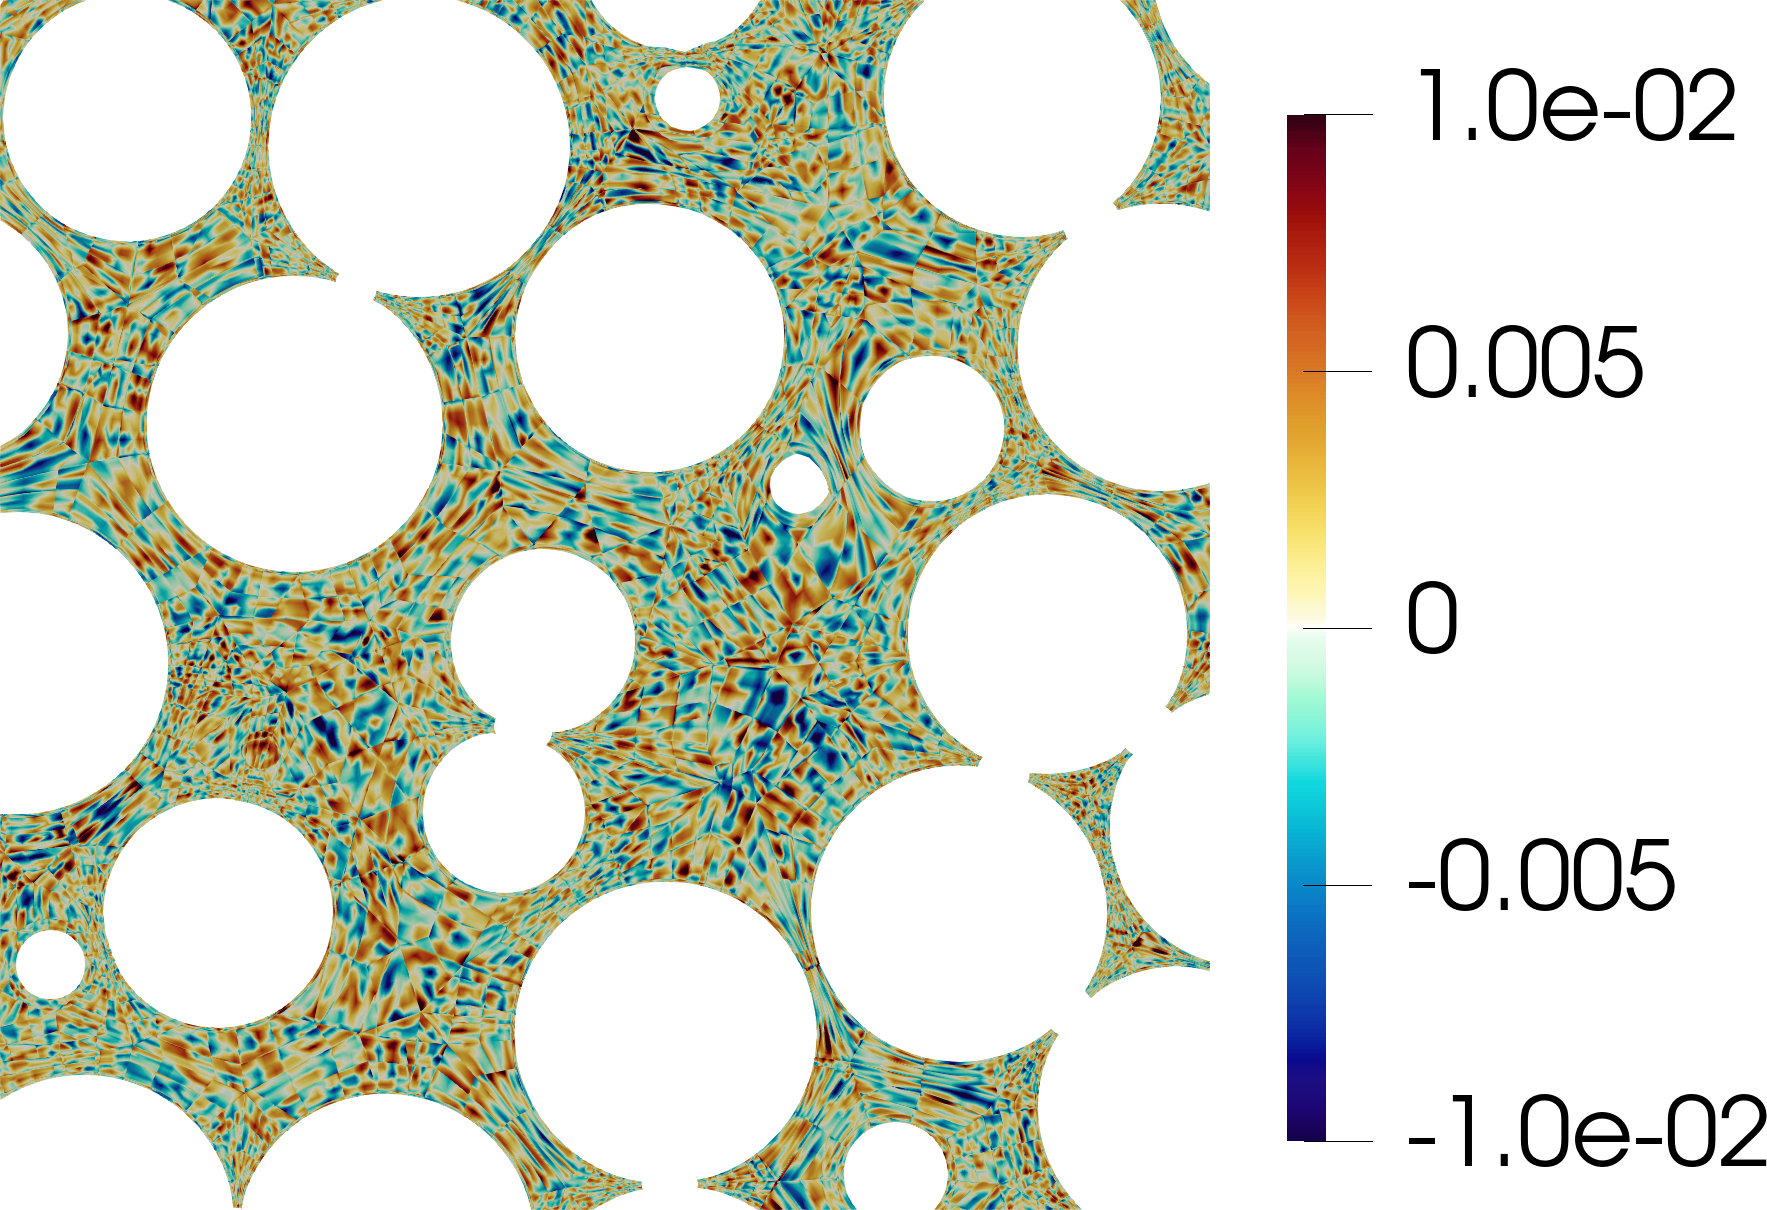
\includegraphics[width=\linewidth]{figs/7/zfp err.png}
    \caption{ZFP}
  \end{subfigure}
  \hfill
  \begin{subfigure}[t]{0.30\linewidth}
    \centering
    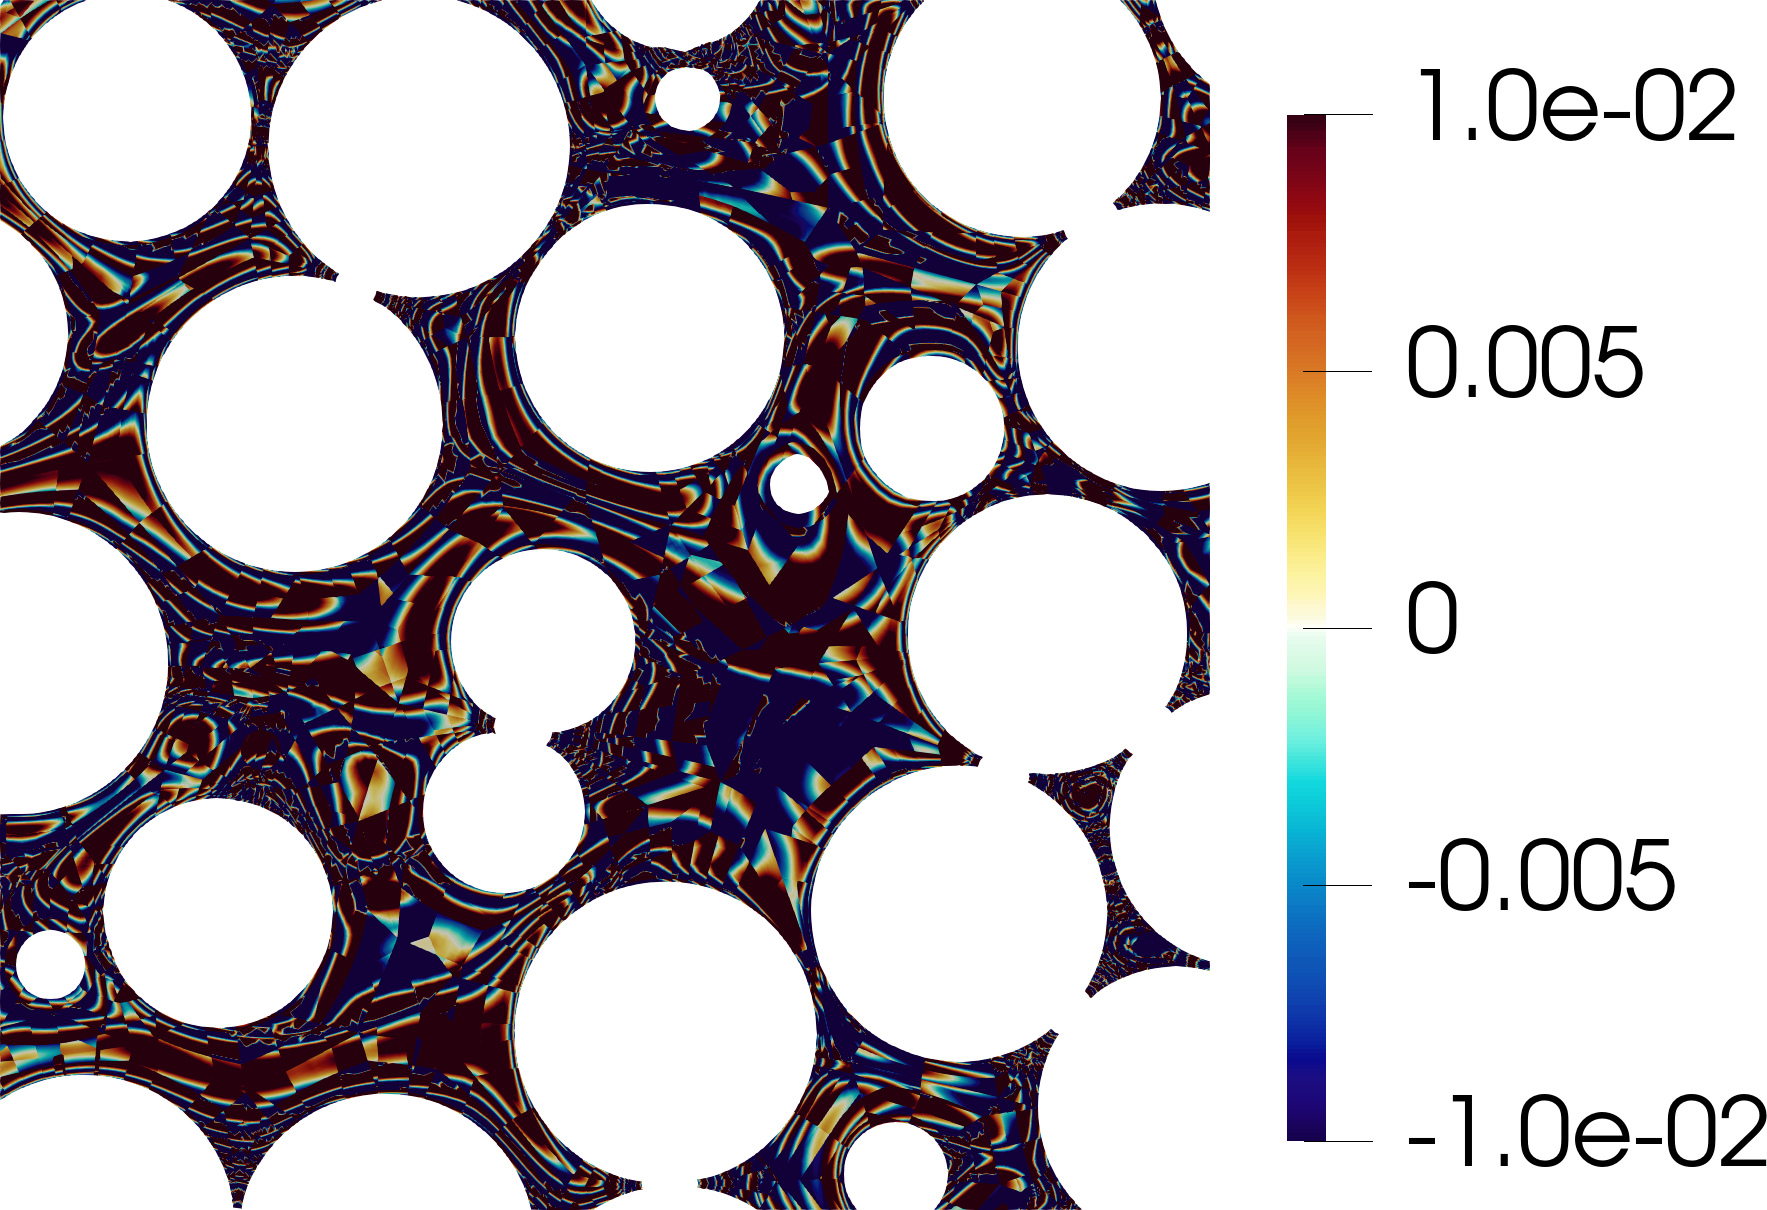
\includegraphics[width=\linewidth]{figs/7/sperr err.png}
    \caption{SPERR}
  \end{subfigure}
  \caption{Difference visualization of a slice of the Temperature field from data 4T. The compression ratios for all compressors are unified as $\sim$26.07 for a fair comparison.}
  \label{fig:distortion}
\end{figure}

Table~\ref{tab:error-bound-visualization} reports the error bounds selected for each compressor to achieve comparable compression ratios of approximately 26.07. Among the evaluated methods, MRCZ requires the tightest value-range-based relative error bound of $1.04\times10^{-4}$, whereas ZFP and SPERR require substantially larger error bounds of $3.16\times10^{-1}$ and $4.52\times10^{-2}$, respectively.

The corresponding pointwise reconstruction errors are visualized in Figure~\ref{fig:distortion}. MRCZ achieves the highest reconstruction fidelity, followed by SZ3-HOHS, while the baseline compressors exhibit more extensive errors.
% 考虑在6.4加一个示例图
% 解释为什么DChT更好
% 更新 acknowledgment
% 分析gll有通用性
% 写更多sz3-hohs的参数

\section{Conclusion and Future Work}\label{sec:conclusion}

High-order hybrid-structured (HOHS) discretizations are widely used in scientific and engineering domains to support high-fidelity simulations. The resulting datasets combine local tensor-product structure with globally unstructured element connectivity, posing distinct challenges for efficient storage and data movement. Existing error-bounded lossy compressors are not designed for this hybrid organization and often struggle to jointly achieve high compression ratios, strict error control, and high throughput.

To address these challenges, we develop two complementary compressors, SZ3-HOHS and MRCZ, within a unified element-local framework with strict pointwise error guarantees. SZ3-HOHS extends the SZ-family pipeline with distance-aware linear interpolation for non-uniform nodal layouts. MRCZ employs prediction based on model representations and enhances compressibility through transform selection, coefficient quantization, and coefficient-layout reorganization. Both methods employ parallel element-centric processing while avoiding costly cross-element dependencies.

Experiments on large-scale HOHS datasets from multiple simulation software packages demonstrate substantial benefits for both storage reduction and end-to-end data movement. At comparable reconstruction quality, SZ3-HOHS improves compression ratios by up to 1.5× over the best-performing baseline, while MRCZ further improves compression effectiveness, reaching compression ratios up to 5.5× those of SZ3-HOHS. In end-to-end data-movement experiments, SZ3-HOHS achieves the shortest overall time, while MRCZ remains competitive through greater data reduction. Both methods also provide high compression and decompression throughput and exhibit strong OpenMP scalability.

% Future work will explore additional invertible and numerically stable transforms beyond the Chebyshev-based transform used in this study, as well as GPU implementations to improve throughput and scalability on heterogeneous systems.

Future work will investigate a broader range of invertible and numerically stable transforms beyond the Chebyshev-based transform adopted in this study. We also plan to develop GPU implementations of SZ3-HOHS and MRCZ to accelerate their prediction, quantization, transform, and lossless-encoding stages, thereby improving throughput and scalability on modern heterogeneous computing platforms.

\begin{acks}
This research was supported by the U.S. Department of Energy, Office of Science, Advanced Scientific Computing Research (ASCR), under contract DE-AC02-06CH11357, and supported by the National Science Foundation under Grant OAC-2311875, OAC-2514036, OAC-2513768, OAC-2330367, OAC-2311756, and OAC-2313122. 
This research used resources of the Argonne Leadership Computing Facility, which is a U.S. Department of Energy Office of Science User Facility operated under contract DE-AC02-06CH11357.
We acknowledge the computing resources provided on Bebop, operated by the Laboratory Computing Resource Center at Argonne National Laboratory, and the ACCESS Anvil system, operated by Purdue University.
\end{acks}

%\clearpage

\bibliographystyle{ACM-Reference-Format}
\bibliography{reference}

\end{document}
\endinput
